% % *** UNUSED ***
% \chapter{Introduction}
% In computer science, machine learning is a set of methods for learning models from examples that accurately perform tasks on new or unseen data without explicitly codifying all instructions. This automation of programming provides a time- and cost-effective alternative to otherwise manually created software solutions, making machine learning popular and widely used for many applications.

% However, the relative lack of human supervision in their creation makes it hard to fully understand the inner workings of trained models and limits the ability to verify that the models work correctly. Even though it is possible to statistically verify the correctness of a model by testing it against an unseen dataset whose ground truth is known, models can unknowingly utilize latent variables that should not be used. Knowledge about those factors is often implicit in the domain of the task and not encoded in the data nor the model. Human expertise is needed to detect and encode them explicitly or to block them out.

% For example, Caruana~\etal\cite{Caruana:2015:IMH:2783258.2788613} built a Generalized Additive Model with pairwise interaction ($GA^2M$) to predict mortality risk for hospitalized patients with pneumonia, a potentially life-threatening lung infection. This area of machine learning is called predictive modeling and uses machine learning to predict a certain outcome, in this case mortality risk, based on values of several input features, in this case laboratory measurements, comorbidities, or patient demographics, and is trained from and applied to many instances. It is not feasible to individually check each prediction of the model manually. However, the machine learning algorithm GA2M used for this study is an intelligible model, that sacrifices parts of its predictive quality in favor of being understandable by humans. This enabled the authors to inspect how features contributed to the predicted outcome. One of their findings was that the model associated having asthma, a chronic lung disease, with a lower mortality rate for pneumonia patients. However, this combination of diseases is known to have a significantly \emph{increased} mortality rate. The authors double checked their data and found that this phenomenon actually occurred in their dataset and thus appeared as correct prediction in their model. After further investigation it became clear that this bias in the dataset stemmed from patients, with those conditions, being treated with intensive care thus lowering their mortality risk below the average. Outside of a hospital the risk of those patients would have been significantly higher. The model, however, only learnt about hospitalized patients which led to it being confident in this false association.

% The above example illustrates the need for human understanding and supervision in machine learning and the incorrect correct result could easily be identified since the authors used a special, intelligible, model. However, not all models used in machine learning are, or even attempt to be, easily interpretable by human experts. To counteract this, visual analytics has been successfully used to visualize machine learning processes in order to understand and gain insights into predictive models. Visual analytics is the area of studying interactive graphical representations of abstract information with the help of computational and statistical procedures, in order to effectively analyze complex data. With regards to understanding the decision making of predictive machine learning models, there are two main strategies: white-box and black-box analysis \cite{class_signatures}.

% In white-box analysis the main focus lies in communicating the internal structure of the model at hand. That is, the analysis is based on the assumption that knowing the full internal state of a model and being able to manually retrace decisions made by it, helps understanding the \emph{behavior} of the model in general.

% In this work we will focus on black-box analysis whose focus is on communicating external behavior of a model. That is, no information about the model itself is utilized during the analysis but rather typically inferred from observing how the model reacts to carefully crafted inputs. Compared to white-box analysis there are several advantages.

% As white-box analysis relies on the internal structure and thus the nature of a particular model type, such as the $GA^2M$ mentioned above, a method developed for one type might not be applicable to a different type. This limits the usefulness of white-box analysis as every new algorithm demands often an entirely new form of representation. Since black-box analysis is model independent findings are universally applicable.

% Another drawback of white-box analysis is its scalability to the complexity of the model. Many solutions do not sufficiently scale as model become more complex. For example, a decision tree with 5 nodes, often used as example when explaining the technique, can easily be visualized and understood in a node-link representation. This representation fails to help understanding a decision tree with hundreds or thousands of nodes. For black-box analysis the internal complexity of a model is irrelevant.

% On the other hand black-box analysis also has drawbacks. Especially the limited knowledge of the underlying model allows only for an approximate understanding of its behavior as testing the entire input space would be intractable.

% The main goal of this thesis is to explore how model agnostic feature contribution methods can help to gain a holistic understanding of, as well as, insights about predictive models using visual analytics. In three stages, we will show the progression from initial observations, that led us to utilizing black-box analysis, to the eventual use of aggregated instance-level explanations to understand, trust, and verify predictive models. Additionally, we show that our developed visual analytics techniques can be helpful for feature engineering.

% Feature engineering is the task of deciding which features will be collected for a particular machine learning problem and how those features are pre-processed or transformed in order to create favorable model results. It requires both expertise of the problem domain, as well as, experience in picking and manipulating features in "the right way". For the most part, feature engineering cannot be automated and is typically seen as "black-art", since it relies on intuition and creativity of the modeler \cite{Domingos:2012:FUT:2347736.2347755}.

% In the first stage we analyze and compare different feature selection strategies. Feature selection is a pre-processing step that, unlike feature engineering, algorithmically determines the possible predictive impact of a feature. Only the most impactful features are then used as input for the predictive modeling process. This is often necessary as a larger number of features require significantly more training examples to accurately represent the valid input space without losing predictive qualities. As feature selection algorithms use similar statistical tools as many predictive modeling techniques it seems plausible to infer the importance of features in the context of decision making through feature selection in a model agnostic way.

% In our analysis we showed that, depending on the chosen feature selection algorithm, different, mostly distinctive, feature sets are deemed to be important while, at the same time, having no significant impact on predictive performance. Additionally, from the view of a domain expert those feature sets were equally reasonable in the context of the prediction task. This insight led to the conclusion that rankings from feature selection algorithms are not informative enough to provide an understanding of the importance of features in the context of decision making. A more powerful approach, while still being model agnostic, is needed.

% In the second stage we explore the influence of features in the decision making process of predictive models through a technique called partial dependence. Partial dependence computes feature impact on model outcomes by systematically probing the model with artificial inputs. That is, while keeping the rest of the input values the same, the inspected feature assumes all possible values showing the relationship of feature values to the prediction score. Aggregated over all observed instances, the general behavior of the model with respect to a given feature can be inferred. By computing a novel feature importance score from partial dependence relationships unusual and interesting relations can be found quickly without having to inspect all, often several thousand, features.

% Analyzing partial dependency relationships on diabetes prediction models trained on electronic medical records containing patient demographics, diagnoses, medications, and laboratory results, using our method we gained several insights. Firstly, we showed that logistic regression models are not expressive enough to accurately model the complex relationships of certain features to the outcome. Secondly, we found that the model used a proxy variable indicating the number of doctor visits as predictor of the healthiness of a patient. However, this is \empgh{not} a valid predictor. Even though a patient is likely to visit a doctor more often if she is sick, the reverse cannot be said. Lastly, imputation of missing values, using the population average in laboratory results, caused the model to become uncertain close to the normal value range of laboratory tests. Even though the above findings show the effectiveness of the proposed method in helping to understand and gain insights into arbitrary predictive models, a major drawback of using partial dependency is its limitations on extending it to relations of multiple features to the predicted outcome.

% In the third stage, we overcome this limitation by leveraging instance-level explanations. Instance-level explanations are defined as the smallest change, to an instance vector, necessary to change the predicted outcome label. Aggregating over those explanations and statistically analyzing the resulting instance subsets, proves as powerful novel approach for understanding the behavior of a model. Additionally, we propose a workflow that helps identify flaws in the \emph{input data}, used to train and test the model.

% We use this workflow to analyze a predictive modeling problem revolving patient admission to a hospital, of patients in the emergency department of said hospital. Accurately predicting whether a patient eventually gets admitted to the hospital helps reducing costs. The major limiting factor of this prediction task is the need for input features readily, and electronically, available at the earliest point possible. To this extend we initially used features of prescribed medications as this information is immediately available electronically. Our analysis showed that there are clear groups of patients where the predictive model is very helpful. However, there are some groups of patients where it is impossible for the predictive model to make accurate predictions given the provided information. One of those groups is patients receiving Diatrizoate Meglumine, a contrast medium for CAT or PET scans. This medication only indicates that a scan was performed, but does not carry information about the result of the scan. However, the result of the scan is the deciding factor whether a patient needs further care or can get sent home. Thus, with the given information it is impossible for the predictive model to make a decision that performs better than random guessing. Including more information in the form of additional features does indeed help with this problem but pushes the time when a decision can be made further back. One possible solution is to utilize the predictive model only for the confident groups of patients and wait for the doctors’ decisions in other cases. This example illustrates that is not only possible to understand decision making of a predictive model through our method, but also its application and value for feature engineering.

% In addition to those promising results, there is still work to do. It still needs to be shown that the proposed workflow of statistical analysis of instance-level explanations can be successfully applied to other data types than binary feature vectors, such as numerical features or highly redundant features such as found in images. Furthermore, a formalization or taxonomy of common machine learning modeling \emph{errors} in both the modeling and feature engineering steps is needed to fully determine the limitations of the proposed black-box analysis methodologies. This can be achieved by taking a survey with both machine learning and domain experts to get an understanding and relevance of different kinds of those errors.

% % Recently, predictive modeling is more and more used to
% % analyze clinical data. Predictive modeling is a machine
% % learning technique that creates an internal model from
% % given training data and predicts outcomes for
% % further input. Clinical data, in this case, revolves
% % around the timeline of patients. The goal of the models
% % is to predict certain diagnoses early. This is a challenging
% % task for medical doctors, since early indicators are not always
% % known or difficult to detect in presence of other medical
% % conditions and many details may have an impact on the
% % final diagnosis.

% % On the other hand, the complexity of the input data makes
% % the task challenging for predictive modeling as well.
% % Traditionally, the input for machine learning algorithms
% % is tabular data. For example, in predictive modeling
% % rows are samples and columns are features. The predicted
% % feature is an additional column. In the case of clinical
% % data, every patient is represented as some tabular
% % features (\eg gender, ethnics, age, etc.) and the actual
% % patient timeline which consists of a list of events
% % associated with a timestamp. The events can be diagnoses
% % a doctor made, procedures that were ordered, laboratory
% % tests that were performed, or medications that were prescribed.
% % Those events cannot be simply treated as tabular data.

% % In order to create good algorithms for creating predictive models
% % it is crucial for researchers to understand and interact with
% % the data. This is where visual analytics comes into play.
% % There are four major tasks that can be addressed by using
% % visual analytics:

% % \begin{enumerate}
% % \item Understanding the data
% % \item Easing interaction with the data
% % \item Understanding the results of the algorithms
% % \item Verifying the integrity and quality of those results (debugging)
% % \end{enumerate}

% % Visual analytics can improve working with almost every step
% % in the predictive modeling pipeline as described in
% % \chapref{chap:pmp} and beyond.
% % The authors are working on several
% % projects where visual analytics improves the workflow of
% % predictive modeling researchers and can lead to new
% % insights.
% % Two notable projects are, firstly, a visualization of the patient
% % data which is described in \chapref{chap:ptv}.
% % While not being directly part of the predictive modeling
% % pipeline this visualization helps creating a mental model
% % of the patient data for the predictive modeling researchers,
% % leading to better assumptions which can
% % be implemented in the predictive modeling algorithms
% % to improve the results.

% % The second project, \infuse , is an interactive system to analyze
% % the results of both feature selection algorithms and
% % classification algorithms, and provides an interface for
% % manually creating feature sets.
% % As described in \chapref{chap:infuse}
% % this project covers the three last steps of the
% % predictive modeling pipeline, cross-validation, feature
% % selection, and classification.

% % Furthermore, the first step of the predictive
% % modeling pipeline can be improved by utilizing
% % a visual query system to create the patient cohort.

% % In \chapref{chap:relwork} we explore some related work
% % and conclude in \chapref{chap:conclusion}.

% \chapter{Predictive Modeling of Medical Data}
% \label{chap:pmp}
% \section{Data Description}
% The clinical data used in our context consists of
% a set of patient histories.
% In addition to general attributes of patients,
% like gender, age, or ethnics, the data consists of
% the patient's history as events in a time series.
% Every event is associated with a timestamp and a type.
% The main types are ``diagnosis", a diagnosis made by a doctor,
% ``procedure", a procedure that was ordered for the patient,
% ``lab-test", a laboratory test that was ordered,
% and ``medication" that was prescribed for the patient.
% The actual type of an event is then for example the actual
% diagnosis in question.
% Event types follow a hierarchy with the main types as roots
% and can be arbitrarily deep depending on the granularity of
% the data (usually up to maximal four levels).
% In the following we call the main type of an event overall type
% and leafs of the hierarchy tree actual types.
% Events can also have attached meta-data, \eg the results
% of a laboratory test along with information whether the
% results were in the range of, below, or above the expected
% value.

% \begin{figure}
% 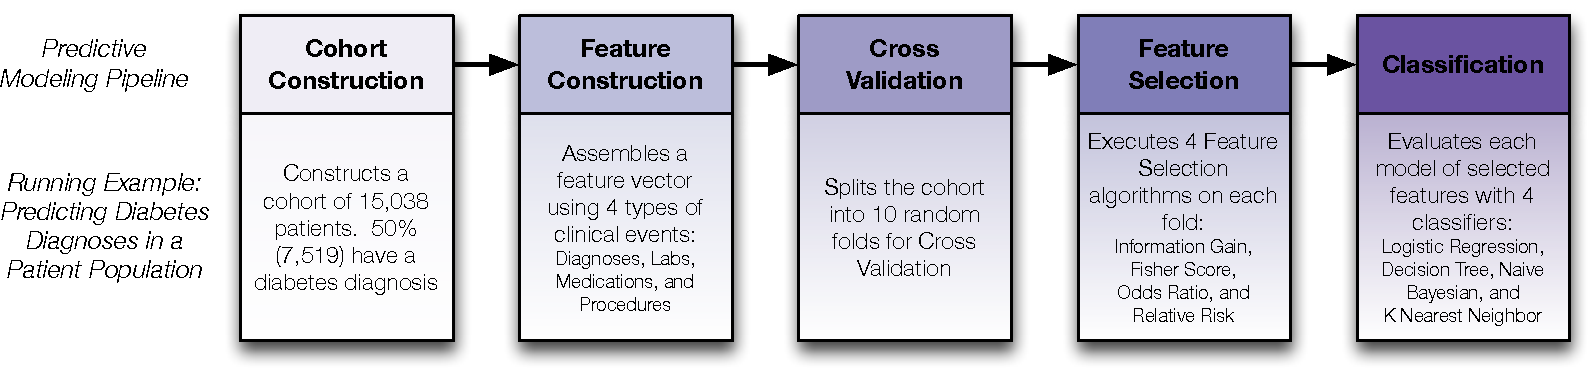
\includegraphics[width=\textwidth]{img/pipeline}
% \caption{
% The predictive modeling pipeline. The first step is to define
% sets of patients (\ie a cohort) for the upcoming tasks.
% Feature construction, the second step, converts the complex
% patient data into features usable by the following
% steps in the pipeline. Cross validation
% splits the patient cohort into folds for verifying the quality
% of the predictions. The fourth step selects a subset of
% features with high predictive value and the last step
% uses those feature sets for classification.
% }
% \label{fig:pipelin}
% \end{figure}

% \section{Predictive Modeling Pipeline}
% In order to build a predictive model for this type of data,
% the following pipeline is used.
% At first, the cohort gets constructed by dividing the set
% of patients into ``cases" and ``controls",
% of which the case patients are eventually diagnosed with
% the to be predicted diagnosis and the control patients
% do not have this diagnosis.
% After that, features are constructed by converting
% the event timelines into features that can be
% used as input to the machine learning algorithms in later steps.
% In order to verify the quality of the predicted outcomes,
% the cohort is split up into cross-validation folds.
% For every cross validation fold, a predictive
% model is created from the remaining set of patients
% and verified with the set of patients in this fold.
% A predictive model is created by first selecting a subset of
% the features via a feature selection algorithm and
% then creating the actual model with a classification algorithm.

% \section{Prediction Quality}
% The quality of the created models is generally measured
% with the area under curve (AUC).
% This is the area under the function of the false positive rate
% (one minus specifity) to the true positive rate (sensitivity)
% \ie the receiver operating characteristic (ROC) curve.
% An area of one is a perfect classification whereas an area
% below $0.5$ suggests negating all predictions in order to
% get a better result.

% \chapter{Patient Timeline Visualization}
% \label{chap:ptv}
% \section{Problem Statement}
% Working with patient data in the form described
% in \chapref{chap:pmp} can be a challenging task.
% When looking at patient histories in chronological order
% important patterns may be overlooked and gaining insight
% into the data becomes difficult.
% This is due to the huge number of events and the fact that
% recurring patterns happen too far from each other to be
% easily detected.
% Even considering those disadvantages, looking at the data
% as chronologial list of events is common practice among
% predictive modelers.
% An example to this can be seen in Figure~\ref{fig:patient_old}.
% Questions researchers want to get answered include
% ``\textit{Are there any patterns in the patient's history?}",
% ``\textit{Are there patterns that patients have in common?}",
% ``\textit{Can those patterns be useful to predict certain diagnoses
% early?}", and
% ``\textit{How does the patient's timeline change after being
% diagnosed with a certain diagnosis?}".

% \begin{figure}
% \centering
% 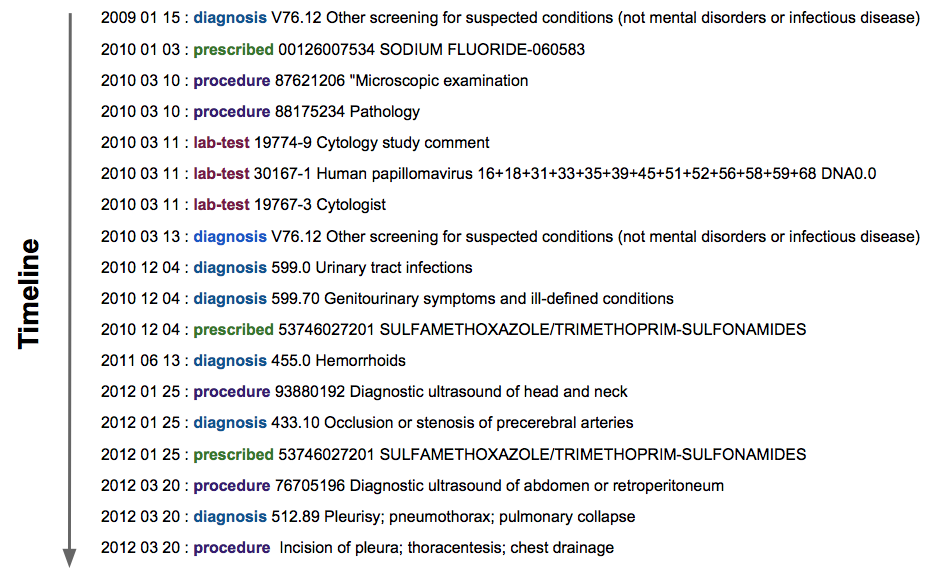
\includegraphics[width=0.5\linewidth]{img/old_timeline}
% \caption{
% The previous way of looking at a patient's history.
% All events in the timeline are chronologically shown in the list.
% }
% \label{fig:patient_old}
% \end{figure}

% \section{Design}
% An improvement to the list representation can be seen in
% Figure~\ref{fig:patient_vis}.
% In this visualization every dot is a particular
% event in the patient's timeline.
% Its color indicates the overall type of the event (\eg diagnosis)
% while the vertical position is dependent on the actual type of the event,
% \eg all same diagnoses (\eg anxiety disorder) appear on the
% same vertical position. Hovering over a dot reveals its
% event type to the user as a tooltip.
% In addition, the vertical axis is sorted by the first
% occurrence of a particular event in the patient's timeline.
% The earlier a particular event occurred in the
% timeline the lower it appears in the visualization.
% The horizontal position indicates the actual time of an event.
% The spacing between dots can be specified to either reflect the
% actual time passed between two events or be removed showing only
% the relative order of the events in time.
% The visualization allows a zooming and panning interaction
% to enable having a closer look at details.
% Above of the visualization a user can see time independent
% information about a patient(see Figure~\ref{fig:patient_vis}).

% \begin{figure}[t]
% \centering
% 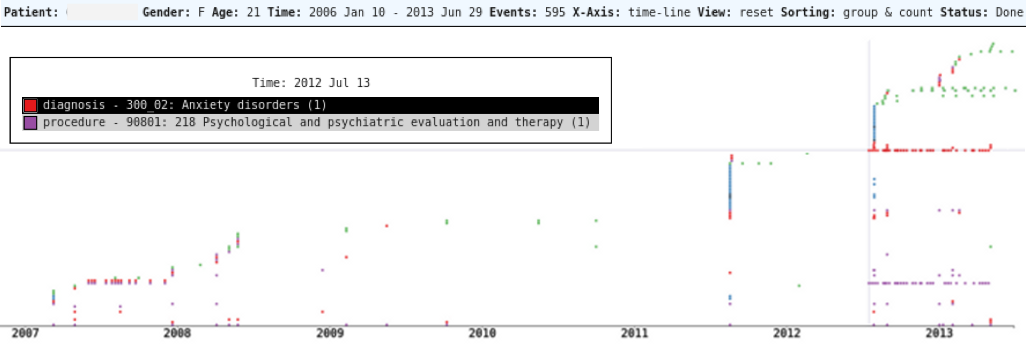
\includegraphics[width=\linewidth]{img/patient_timeline}
% \caption{
% A patient's timeline. The top bar shows time independent
% information of the patient while the center shows events (dots)
% in their chronological order. The vertical position of an event
% indicates its first occurrence. All events of the same type
% are on the same vertical position while color is used to
% distinguish between the overall types
% (see Figure~\ref{fig:sidebar}).
% Currently a first occurrence of a diagnosis is selected.
% The box in the upper left shows all events that happened
% on that day.
% }
% \label{fig:patient_vis}
% \end{figure}

% This way of visualizing a patient's history enables the detection of
% interesting patterns and makes it easier to create a mental model
% of it. For example, in Figure~\ref{fig:patient_vis} the first diagnosis
% of an anxiety disorder is currently selected. The vertical bar indicates
% the date of this as well as the box in the top left corner
% which indicates all events that happened during that day. The horizontal
% bar shows all occurrences of this diagnosis which is repeated for all
% visits to a doctor as long as the diagnosis persists. The two bars
% divide the area into four regions. The lower left corner contains
% all events before the diagnosis, the lower right corner contains
% events that happened after the initial diagnosis which are not new
% after this point in time and the upper right corner contains all
% new events that happened after the initial diagnosis.
% In this case a number of new lab-tests are ordered and the patient
% gets a recurring prescription of some new medication as well
% as a recurring procedure that, however, was performed before.

% The position of the bars can be changed by clicking on the
% visualization. If the user clicks on the white area
% the vertical bar is set to the date represented by the
% given position and the box in the upper left, containing
% all events that happened on that day, is updated.
% Clicking on a dot not only updates the vertical bar but also
% selects the event type of the dot thus moving the horizontal
% bar on its vertical position.

% In addition to the main visualization showing the events in
% order a listing of all distinct event types is provided as well
% (see Figure~\ref{fig:sidebar}).
% This listing is divided into the four overall types which
% also provide a color key for the dots in the main visualization.
% Distinct events can be sorted by their number of occurrences
% showing the most common event types at the top.
% Sorting by name enables users to find a given type faster.
% Event types in the list can be selected which will be
% reflected in the main visualization by changing the position
% of the horizontal bar thus showing where this type of event
% can be found. Selections in either part of the visualization
% are reflected in all views.

% \begin{figure}
% \centering
% 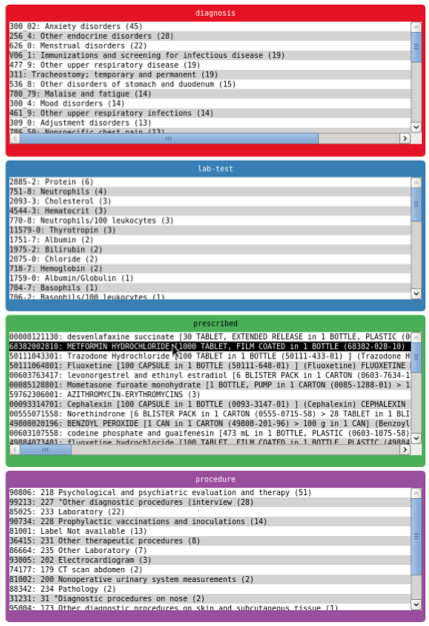
\includegraphics[width=0.35\linewidth]{img/sidebar}
% \caption{
% Lists of all distinct events in a patient's history.
% The events are grouped by their overall type (distinguished by
% color) and are sorted by their number of occurrences or by name.
% }
% \label{fig:sidebar}
% \end{figure}

% \section{Conclusion}
% Even though, the project is still in an early stage, the
% predictive modeling researcher's understanding of the
% data has already improved significantly.
% The researchers have included the tool in their daily work-flow
% providing continuous feedback.
% Additional feature requests and improvements for the tool
% still need to be implemented, as the project is still in
% active development.

% \begin{figure}
% \centering
% 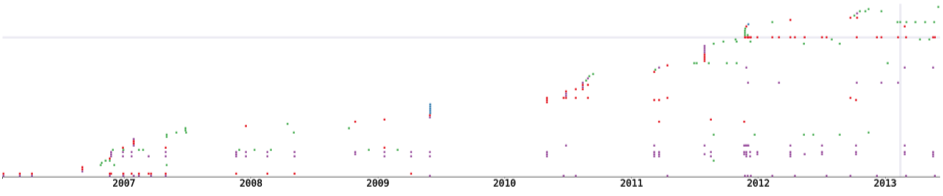
\includegraphics[width=\linewidth]{img/timeline_alt}
% \caption{
% A patient's timeline. Notice the regular doctor visits along
% with procedure subscriptions until 2010. During 2010 the
% patient gets diagnosed some new diagnoses resulting in a
% temporary breaking of the pattern. The procedure subscription
% pattern from the beginning is resumed early 2011 with a
% different pace. Eventually, in 2012 the patient is diagnosed
% with diabetes (the selected line).
% }
% \label{fig:timeline_alt}
% \end{figure}

% \chapter{Interactive Feature Selection (INFUSE)}
% \label{chap:infuse}

% \section{Problem Statement}
% Comparing the quality of multiple feature selection
% and classification algorithms usually is done
% using a single numerical value. By doing this
% information about the internal reasoning of the algorithms
% and intermediate results are thrown away.
% This information, however, is difficult to interpret
% or to compare.
% Potential tasks researchers might want to accomplish
% by interpreting and comparing the results are:

% \begin{description}
% \item[Comparison of feature selection algorithms.] In data sets with thousands of features, it is important to have a quick way to understand how feature selection algorithms rank different features differently. Some of the typical questions researchers ask are: ``\textit{Which features are consistently ranked high by all the algorithms?}"; ``\textit{How much do the algorithms differ in their ranking?}"; ``\textit{Are there features that have a high rank on some algorithms and a low rank on others?}"; ``\textit{How robust are the rankings with respect to different data samples?}"

% \item[Comparison of classification algorithms.] The output of each feature selection algorithm is used to feed a series of classification algorithms. At the end of this process, the user is left with a $F \times C$ number of performance comparisons, where $F$ is the number of feature selection algorithms and $C$ the number of classification algorithms. Typical questions researchers ask are: ``\textit{Which combinations of feature selection and classification algorithms give the best scores?}"; ``\textit{Are there feature selection algorithms that score consistently better across the set of classification algorithms?}"; ``\textit{Are there classification algorithms that score consistently better across the set of feature selection algorithms?}"; ``\textit{Which sets of features are selected in the model(s) that yield the highest performance?}"

% \item[Manual selection and testing of new feature sets.] Related to the last question of the previous task, researchers see value in being able to add or remove features of interest from models. This is desired because there can be additional domain-relevant knowledge, beyond model performance, to introduce a desired feature or remove an undesired one.  Typical questions researchers ask are: ``\textit{How does the performance of the model increase or decrease if I remove or add these features?}"; ``\textit{How does a new model compare to the models automatically built by the system?}"; ``\textit{Can feature A
% be replaced by feature B and still yield a similar outcome?
% (For example testing with a cheaper laboratory test instead of
% a more expensive one)}".
% \end{description}

% \infuse is a tool aimed to provide a way to accomplish those
% tasks by visualizing the outcomes of feature selection
% and classification algorithms in the predictive modeling
% pipeline. Interaction techniques and multiple views help
% navigating the shown information and allow for defining
% new models to be analyzed in order to accomplish the third task.
% \infuse provides a user-centric way of manipulating
% predictive models.

% \section{Design}
% The tool is divided into three parts, Feature View, List View,
% and Classification View. The arrangement of those views
% can be seen in Figure~\ref{fig:infuse}. The views are interlinked
% and selections in one view are propagated to the other views.
% In following sections explain in detail how data is represented
% and why the current design was chosen.

% \begin{figure}[t]
% \centering
% 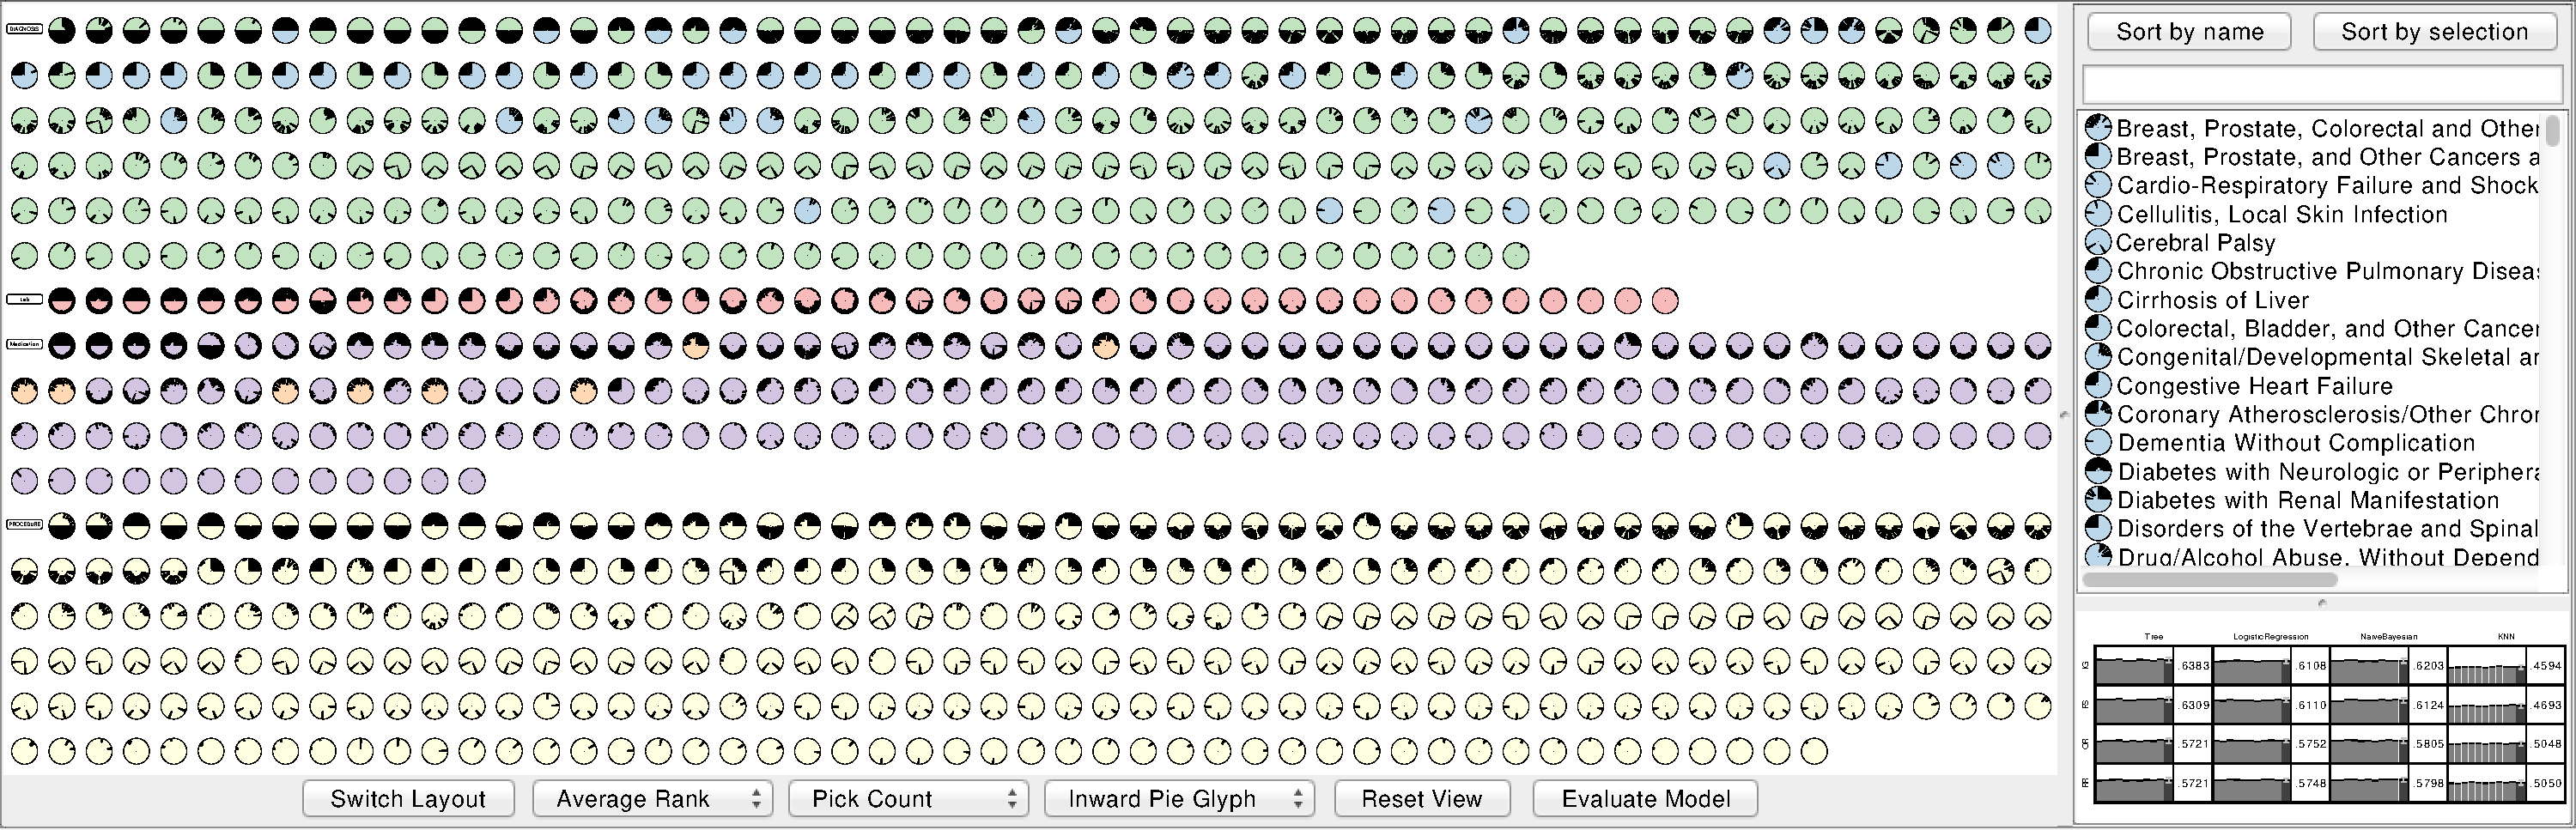
\includegraphics[width=\linewidth]{img/teaser}
% \caption{
% The main interface of \infuse . The center arranges
% feature glyphs which show the importance of features under
% different feature selection algorithms and
% cross-validation folds.
% To the right is a list of all features which can be sorted
% in different ways and in the lower right corner the results
% of the classification algorithms can be seen.
% }
% \label{fig:infuse}
% \end{figure}

% \begin{figure}
% \centering
% 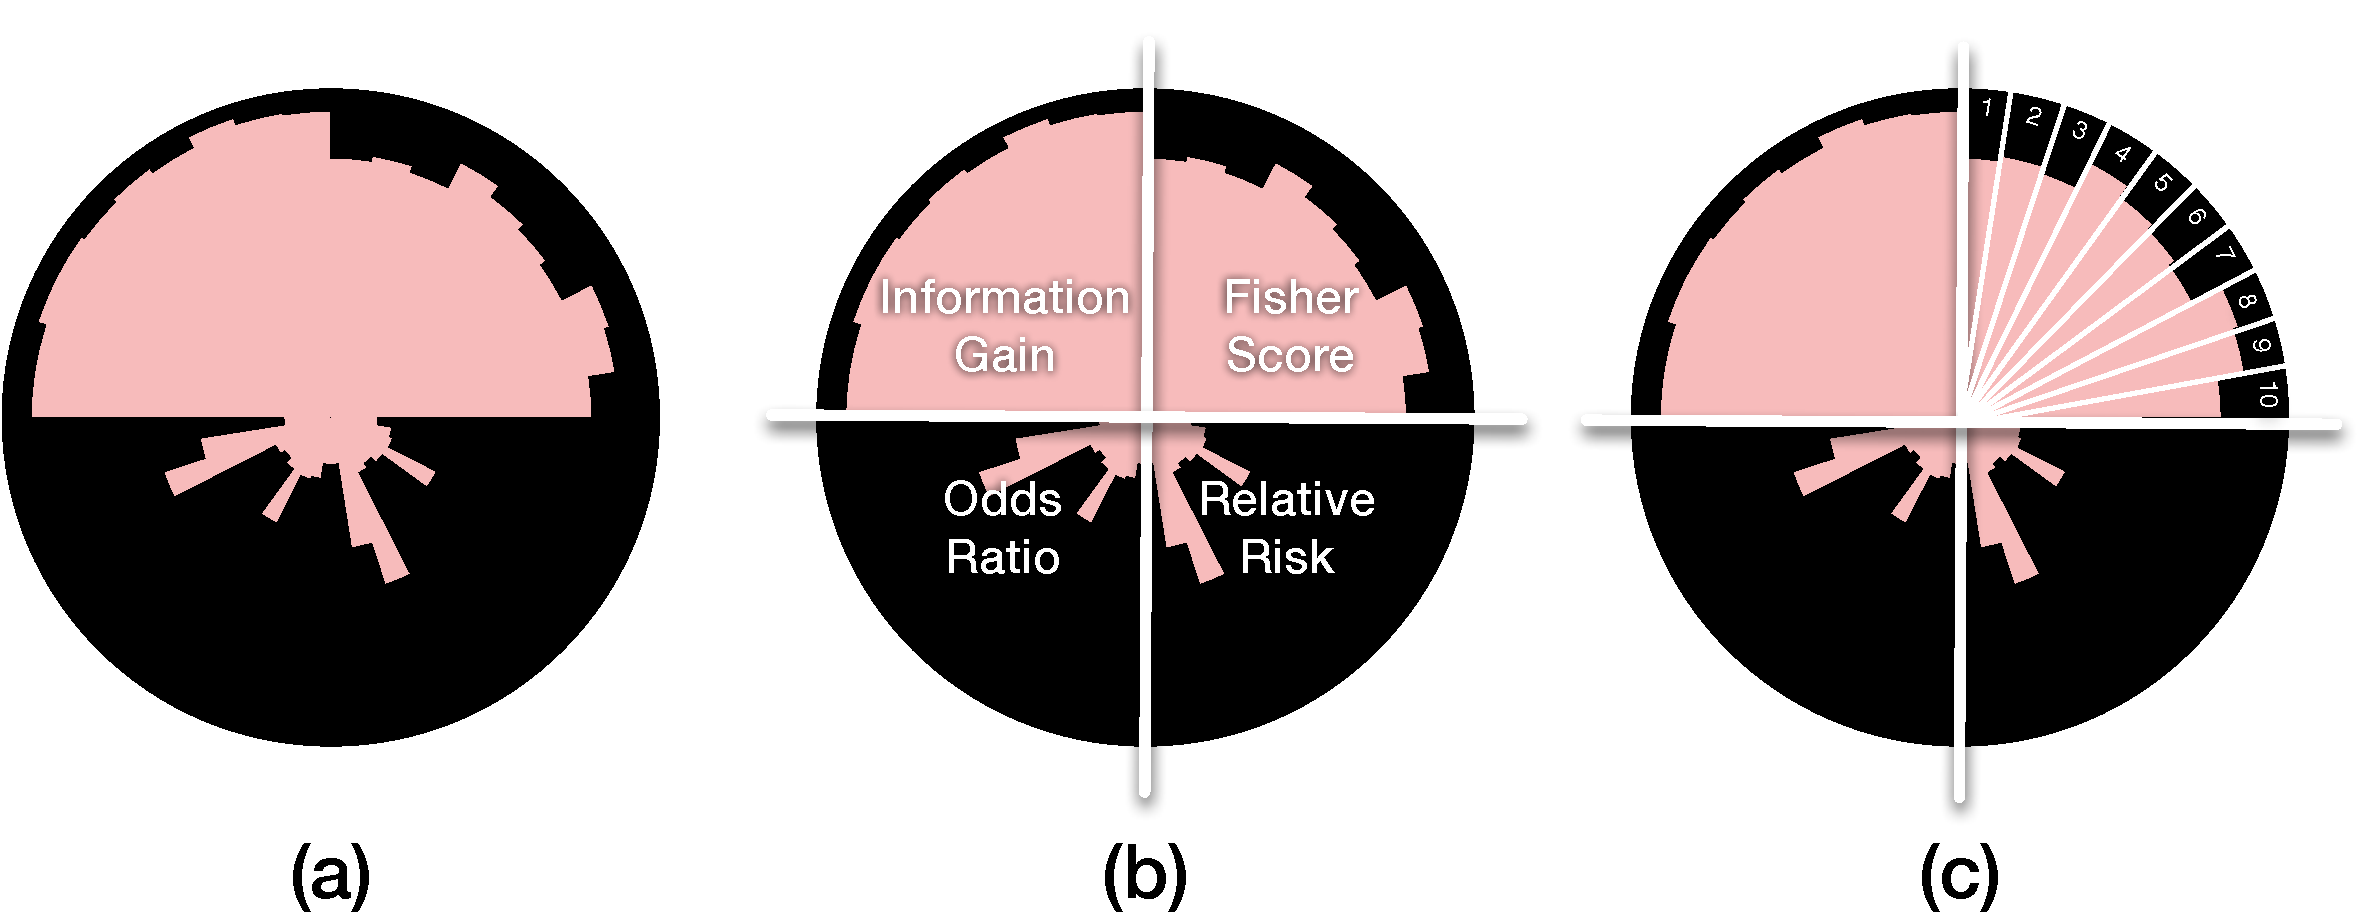
\includegraphics[width=\linewidth]{img/glyph-key}
% \caption{
% The design of the feature glyphs used in \infuse .
% The circle is divided into four regions, one for each
% feature selection algorithm. Those regions are then divided
% into ten slices for every cross-validation fold.
% Within each slice, the rank of the feature for the given
% setting is shown as black bar. The longer the bar, the better
% the ranking. If a bar extends all the way to the middle,
% this feature is considered most important for the given
% feature selection algorithm under the given fold.
% }
% \label{fig:key}
% \end{figure}

% \subsection{Feature View}
% The main part of the tool is the Feature View,
% a zoomable user interface showing
% the results of feature selection algorithms.
% Every feature is represented as glyph showing its performance
% \wrt different feature selection algorithms and within
% different cross-validation folds.
% The glyph (as seen in Figure~\ref{fig:key})
% is split into four sections, one for every
% algorithm, namely Information Gain, Fisher Score, Relative Risk,
% and Odds Ratio. The sections are then further split into
% slices for the ten cross-validation folds.
% Every combination of algorithm and fold results in a
% potentially different rank within the selected feature set
% if the feature was selected.
% This rank is shown as a black bar filling a slice growing
% inwards. The slice is completely empty when the feature
% is unranked, \ie was not chosen by the feature selection
% algorithm for the given cross-validation fold.
% If a feature is ranked the best under a given
% combination of feature selection algorithm and cross-validation
% fold the corresponding slice is completely black.
% This form of representation makes it easier to compare
% features to each other even when features have
% poor ranked slices.

% \begin{figure}
% \subfigure[][]{
% \centering
% 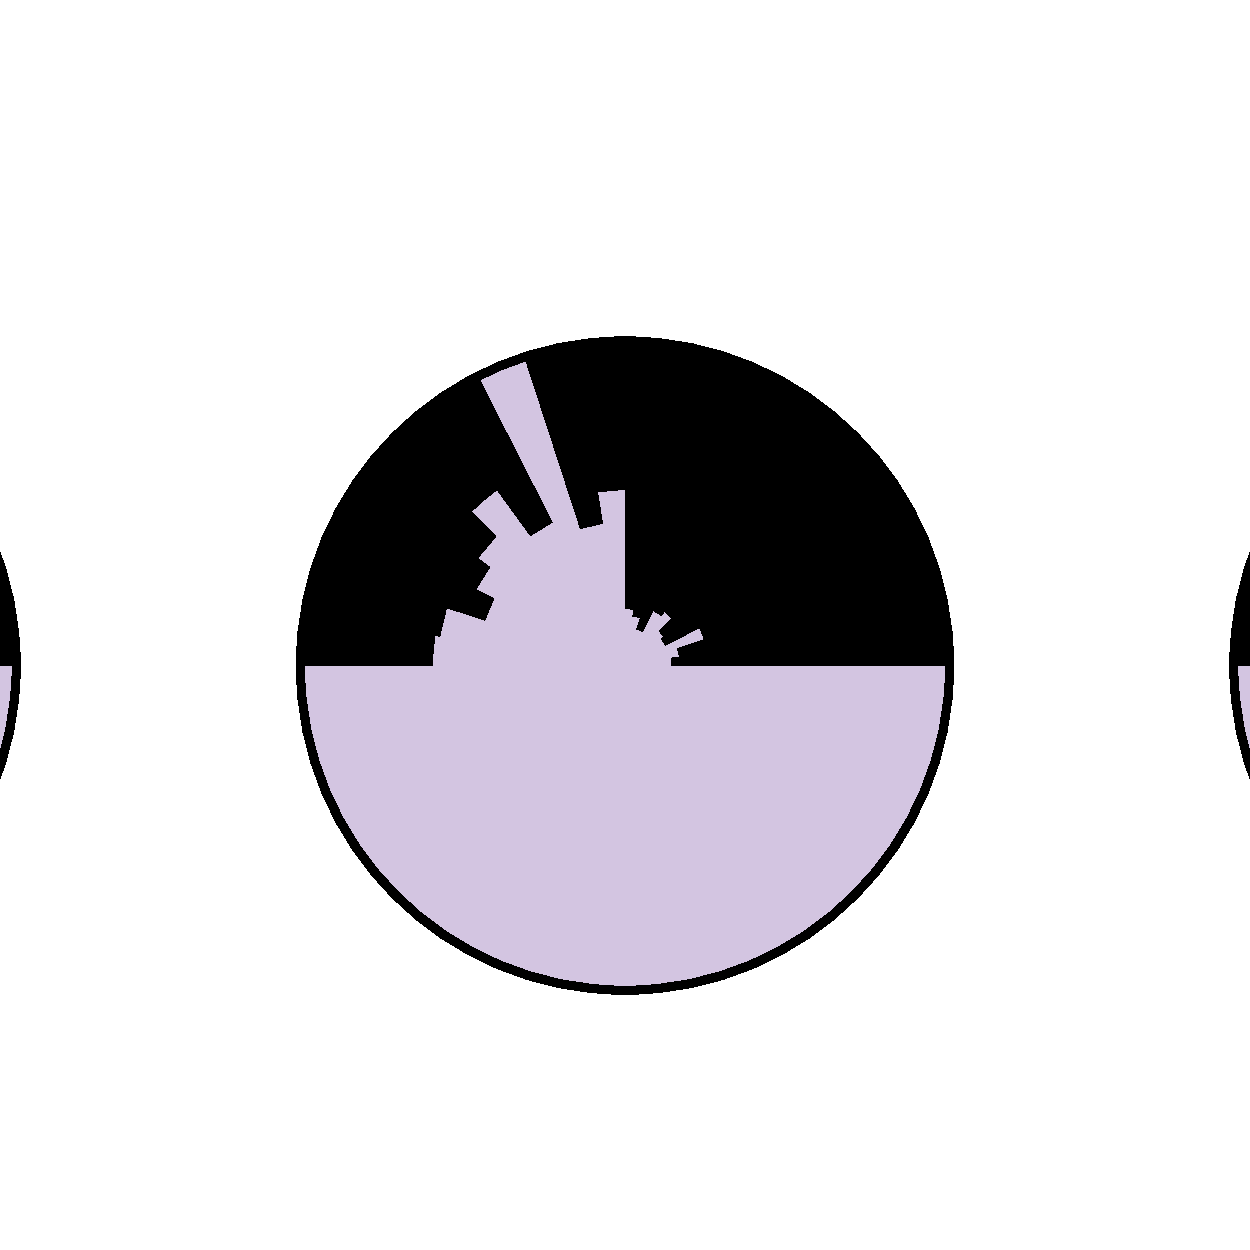
\includegraphics[width=0.23\linewidth,clip,trim={2.4cm 4cm 1.7cm 4cm}]{img/g0}
% \label{subfig:inward}
% }%
% \hspace*{0.01\linewidth}%
% \subfigure[][]{
% \centering
% 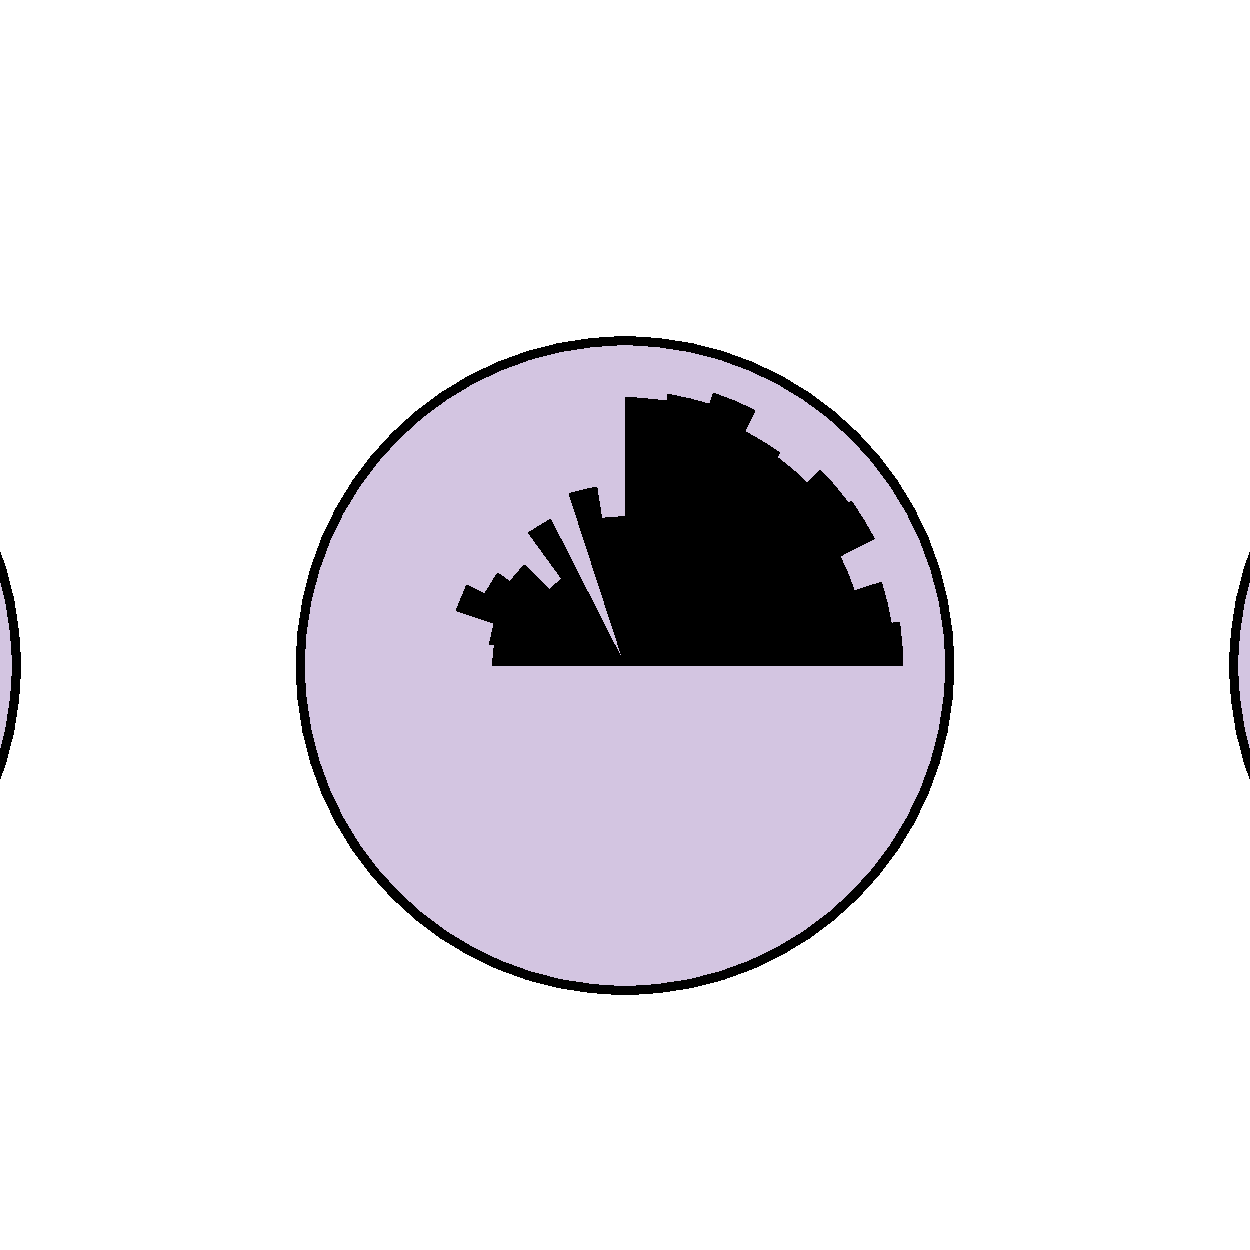
\includegraphics[width=0.23\linewidth,clip,trim={2.4cm 4cm 1.7cm 4cm}]{img/g1}
% \label{subfig:pie}
% }%
% \hspace*{0.01\linewidth}%
% \subfigure[][]{
% \centering
% 
\includegraphics[width=0.23\linewidth,clip,trim={2.4cm 4cm 1.7cm 4cm}]{img/g2}
% \label{subfig:star}
% }%
% \hspace*{0.01\linewidth}%
% \subfigure[][]{
% \centering
% 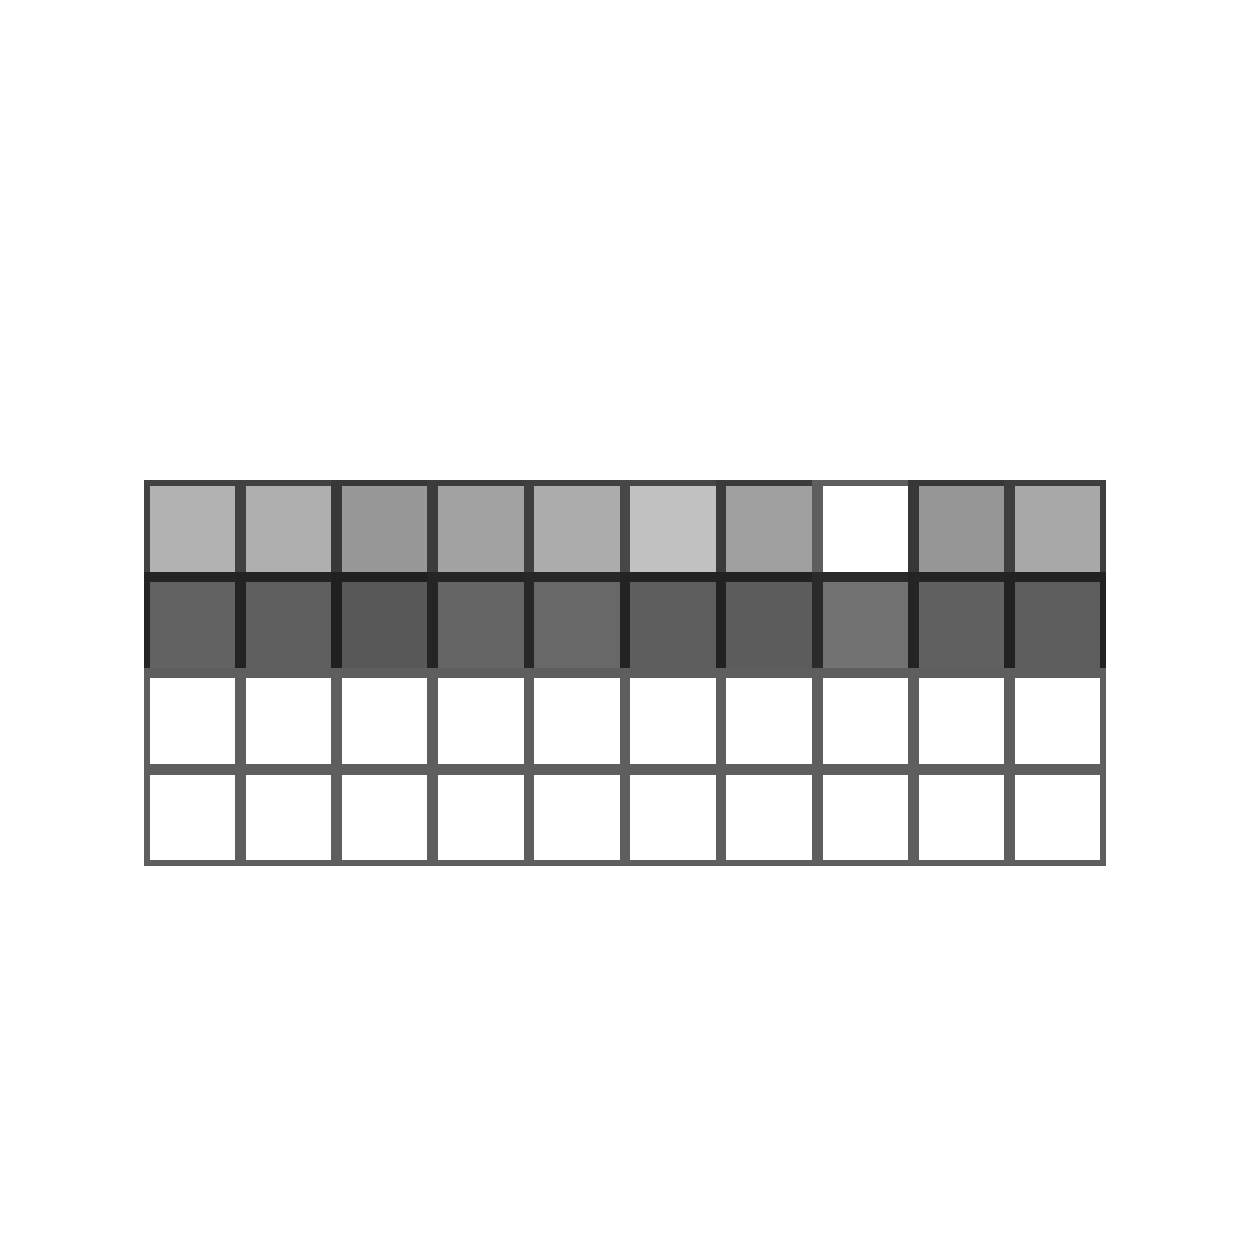
\includegraphics[width=0.23\linewidth,clip,trim={2.4cm 4cm 1.7cm 4cm}]{img/g3}
% \label{subfig:matrix}
% }%
% \caption{
% Different glyph designs.
% \subref{subfig:inward} shows \emph{fold slices} with bars growing from perimeter to center
% whereas \subref{subfig:pie} grows from center to perimeter.
% \subref{subfig:star} shows a typical starburst glyph and
% \subref{subfig:matrix} shows a matrix using luminance to show the ranks.
% Note that in \subref{subfig:pie} and \subref{subfig:star} it is difficult
% to see that this feature is unranked in the third fold from the right in
% the top left quadrant.
% The values in \subref{subfig:star} are difficult to read because
% there is no reference to how big the values are.
% Luminance, as used in \subref{subfig:matrix} is a harder perceptual attribute for users
% to interpret and distinguish than length and area are, as used by the other glyphs.
% }
% \label{fig:glyph_design}
% \end{figure}

% In its development, the glyph design went through several
% stages before reaching its current form.
% Alternatives can be seen in Figure~\ref{fig:glyph_design}.
% Having slices fill up from the inside makes it difficult
% to identify the fold and feature selection algorithm for
% low ranked features.
% The same problem applies to the
% starburst glyph representation which in addition doesn't
% have a reference for how long the bar for the best rank would be.
% The matrix representation uses luminance to show the ranks
% which is inferior to using length thus more
% difficult to interpret.

% In the Feature View features can be selected by clicking on
% them or using a lasso tool.
% Selections are linked throughout all views.
% In addition to selecting features a user can rearrange the
% glyphs according to various
% statistical properties of their ranks as seen
% in Figure~\ref{fig:scatter}.
% Rearranging feature glyphs result in a scatter plot whose
% axes can be defined by the user.
% The choices for axes include:

% \begin{itemize}
% \item the \emph{average rank} of a feature\\
% (ignores unranked slices)
% \item the \emph{pick count} of the number of combined
% feature selection algorithms\\
% and cross-validation folds that picked the feature
% \item the \emph{importance} of a feature
% \item the \emph{best rank} of the feature
% \item the \emph{median rank} of the feature\\
% (ignores unranked slices)
% \item the \emph{standard deviation} of the feature's ranks\\
% (ignores unranked slices)
% \end{itemize}

% The importance of a feature is computed with the following
% formula as average rank with penalties for slices that
% did not choose the feature:
% \[
% rank_{best} = \min_{m \in M \times V, f \in F}{[rank_{m}(f)]}
% \]\[
% i(f) = \dfrac{1}{| M \times V |}[
% 2 \cdot rank_{best} \cdot
% unranked_{M \times V} (f)
% + \sum_{m \in M \times V} rank_{m}(f)
% ]
% \]
% where $M$ is the set of models \ie the feature selection
% algorithms, $V$ is the set of cross-validation folds,
% $F$ is the set of features,
% $rank_{m}(f)$ is the rank of a feature $f$ in the combined model
% and cross-validation fold $m$,
% and $unranked_{M \times V} (f)$ is the number
% of such combined models that did not choose $f$.
% The formula assumes $rank_{m}(f) = 0$ for unranked features $f$
% in the combined model $m$ only when computing $i(f)$.
% Note that a small value for $i(f)$ means higher importance.
% The optimal value is $1$.

% This statistical information about the ranks of a feature
% can be seen when hovering with the mouse over a feature glyph.

% \begin{figure}
% \centering
% \subfigure[][]{
% 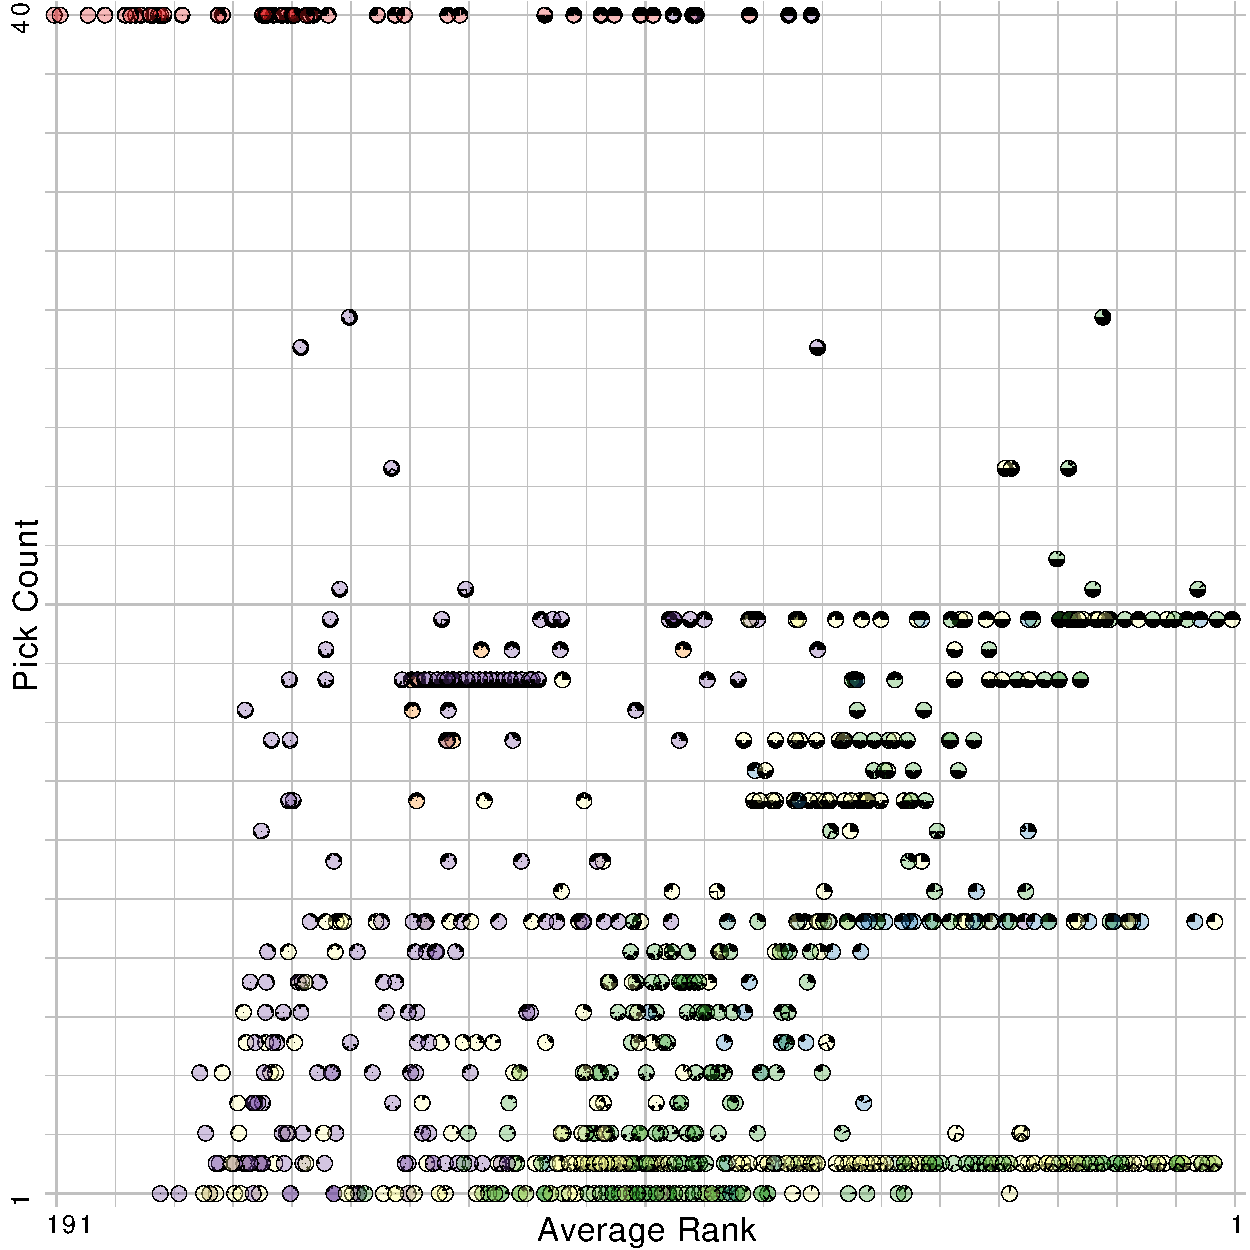
\includegraphics[width=3.42cm]{img/ap}
% \label{subfig:ap}
% }%
% ~%
% \subfigure[][]{
% 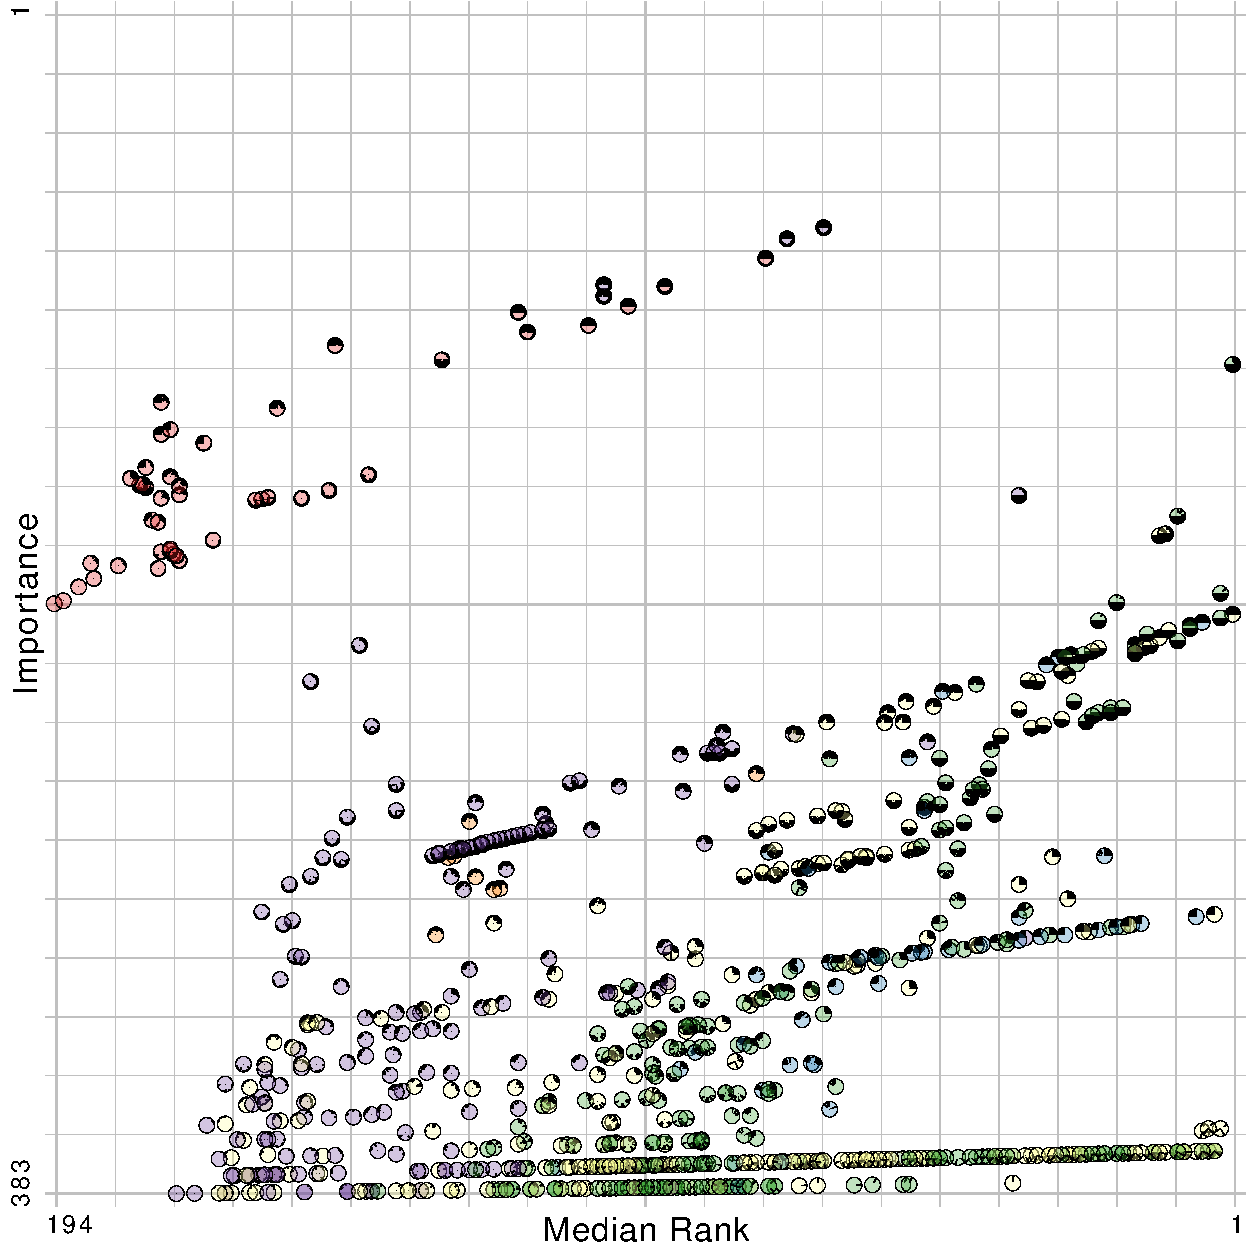
\includegraphics[width=3.42cm]{img/mi}
% \label{subfig:mi}
% }%
% ~%
% \subfigure[][]{
% 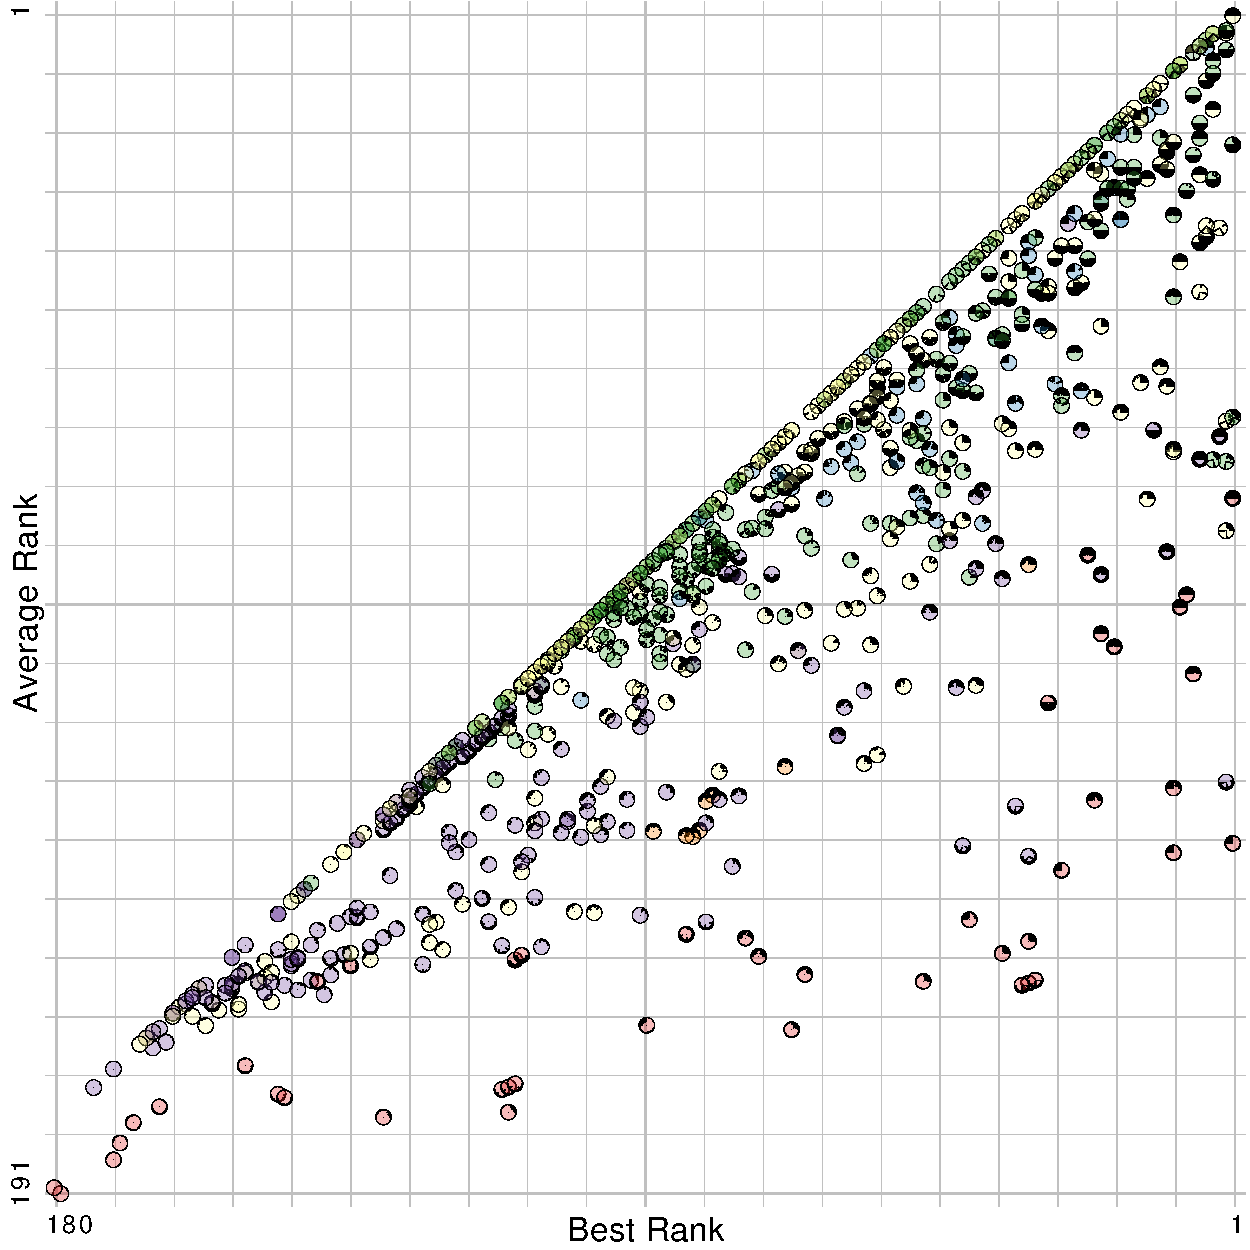
\includegraphics[width=3.42cm]{img/ba}
% \label{subfig:ba}
% }%
% ~%
% \subfigure[][]{
% 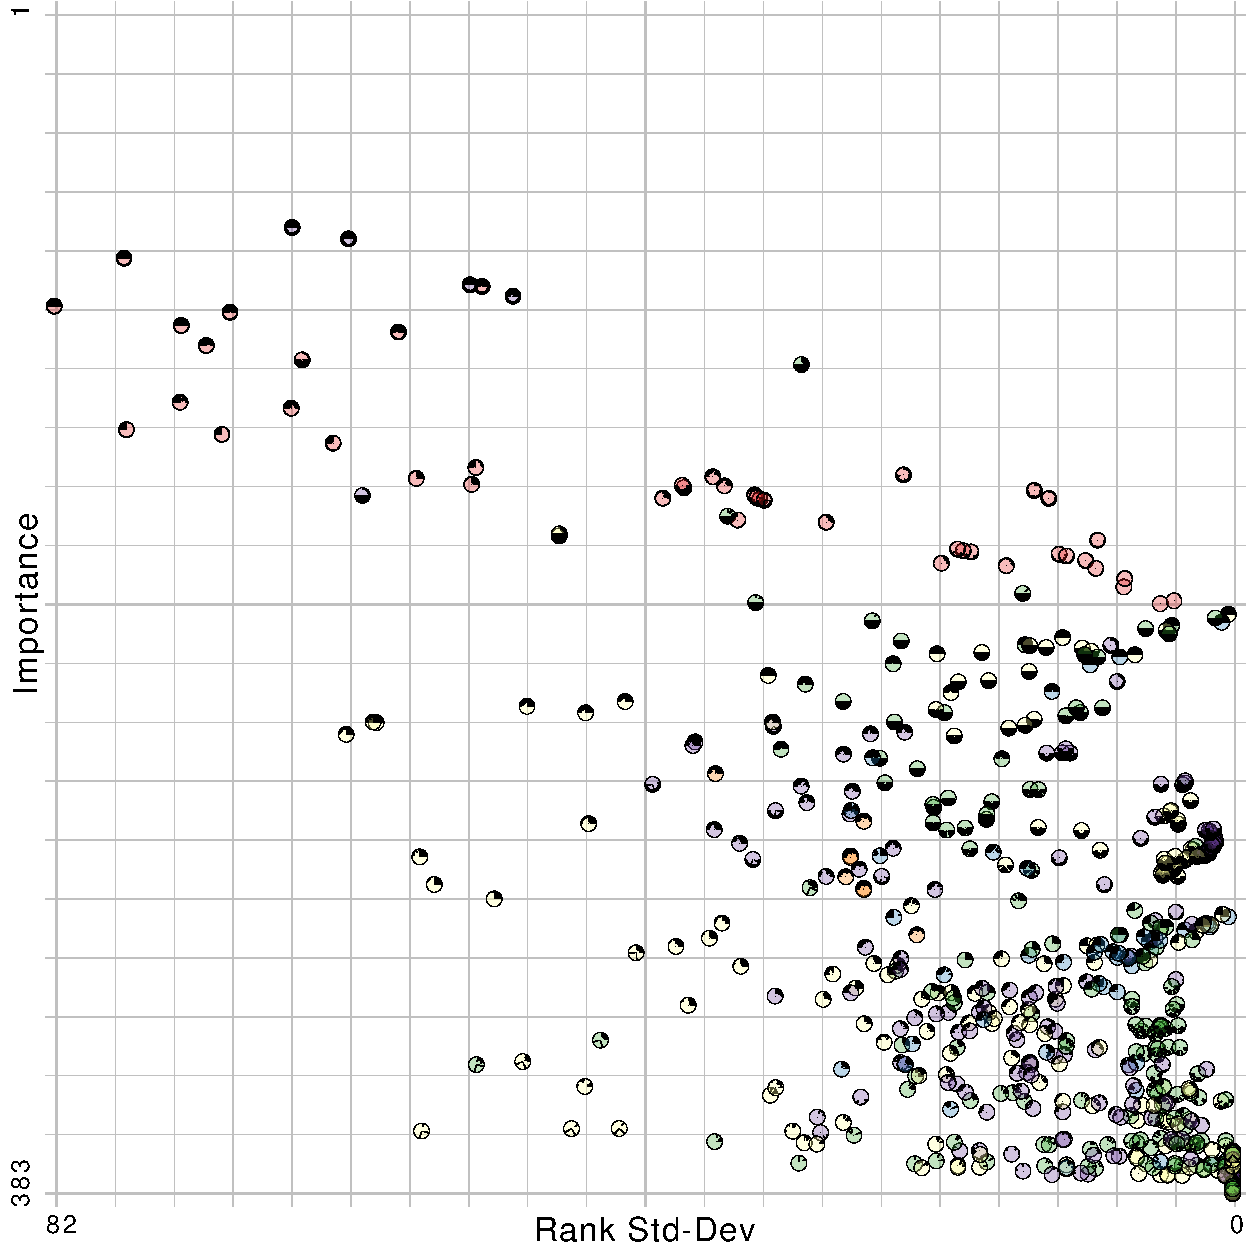
\includegraphics[width=3.42cm]{img/si}
% \label{subfig:si}
% }
% \caption{
% Different axis combinations for the scatter-plot layout.
% In \subref{subfig:ap} the average rank is plotted against the pick count.
% Most of the features appear in the lower half because features are rarely picked by more than two algorithms in this example.  The bottom-right shows features that are only chosen
% by two models but were ranked very high by them.
% \subref{subfig:mi} shows the median rank plotted against the importance.
% Notice that the plot looks similar to \subref{subfig:ap} since importance
% is a combination of the axes from \subref{subfig:ap}.
% The axes in \subref{subfig:ba} are best rank versus average rank.
% Features can only appear below the diagonal.
% The standard deviation of the ranks is plotted against the importance
% in \subref{subfig:si}.
% The peak to the bottom right corner consists of features that are rarely
% picked and therefore have lower variance.
% The peak to the top right consists of features that
% are consistently high ranked.
% }
% \label{fig:scatter}
% \end{figure}

% \begin{figure}[t]
% \centering
% 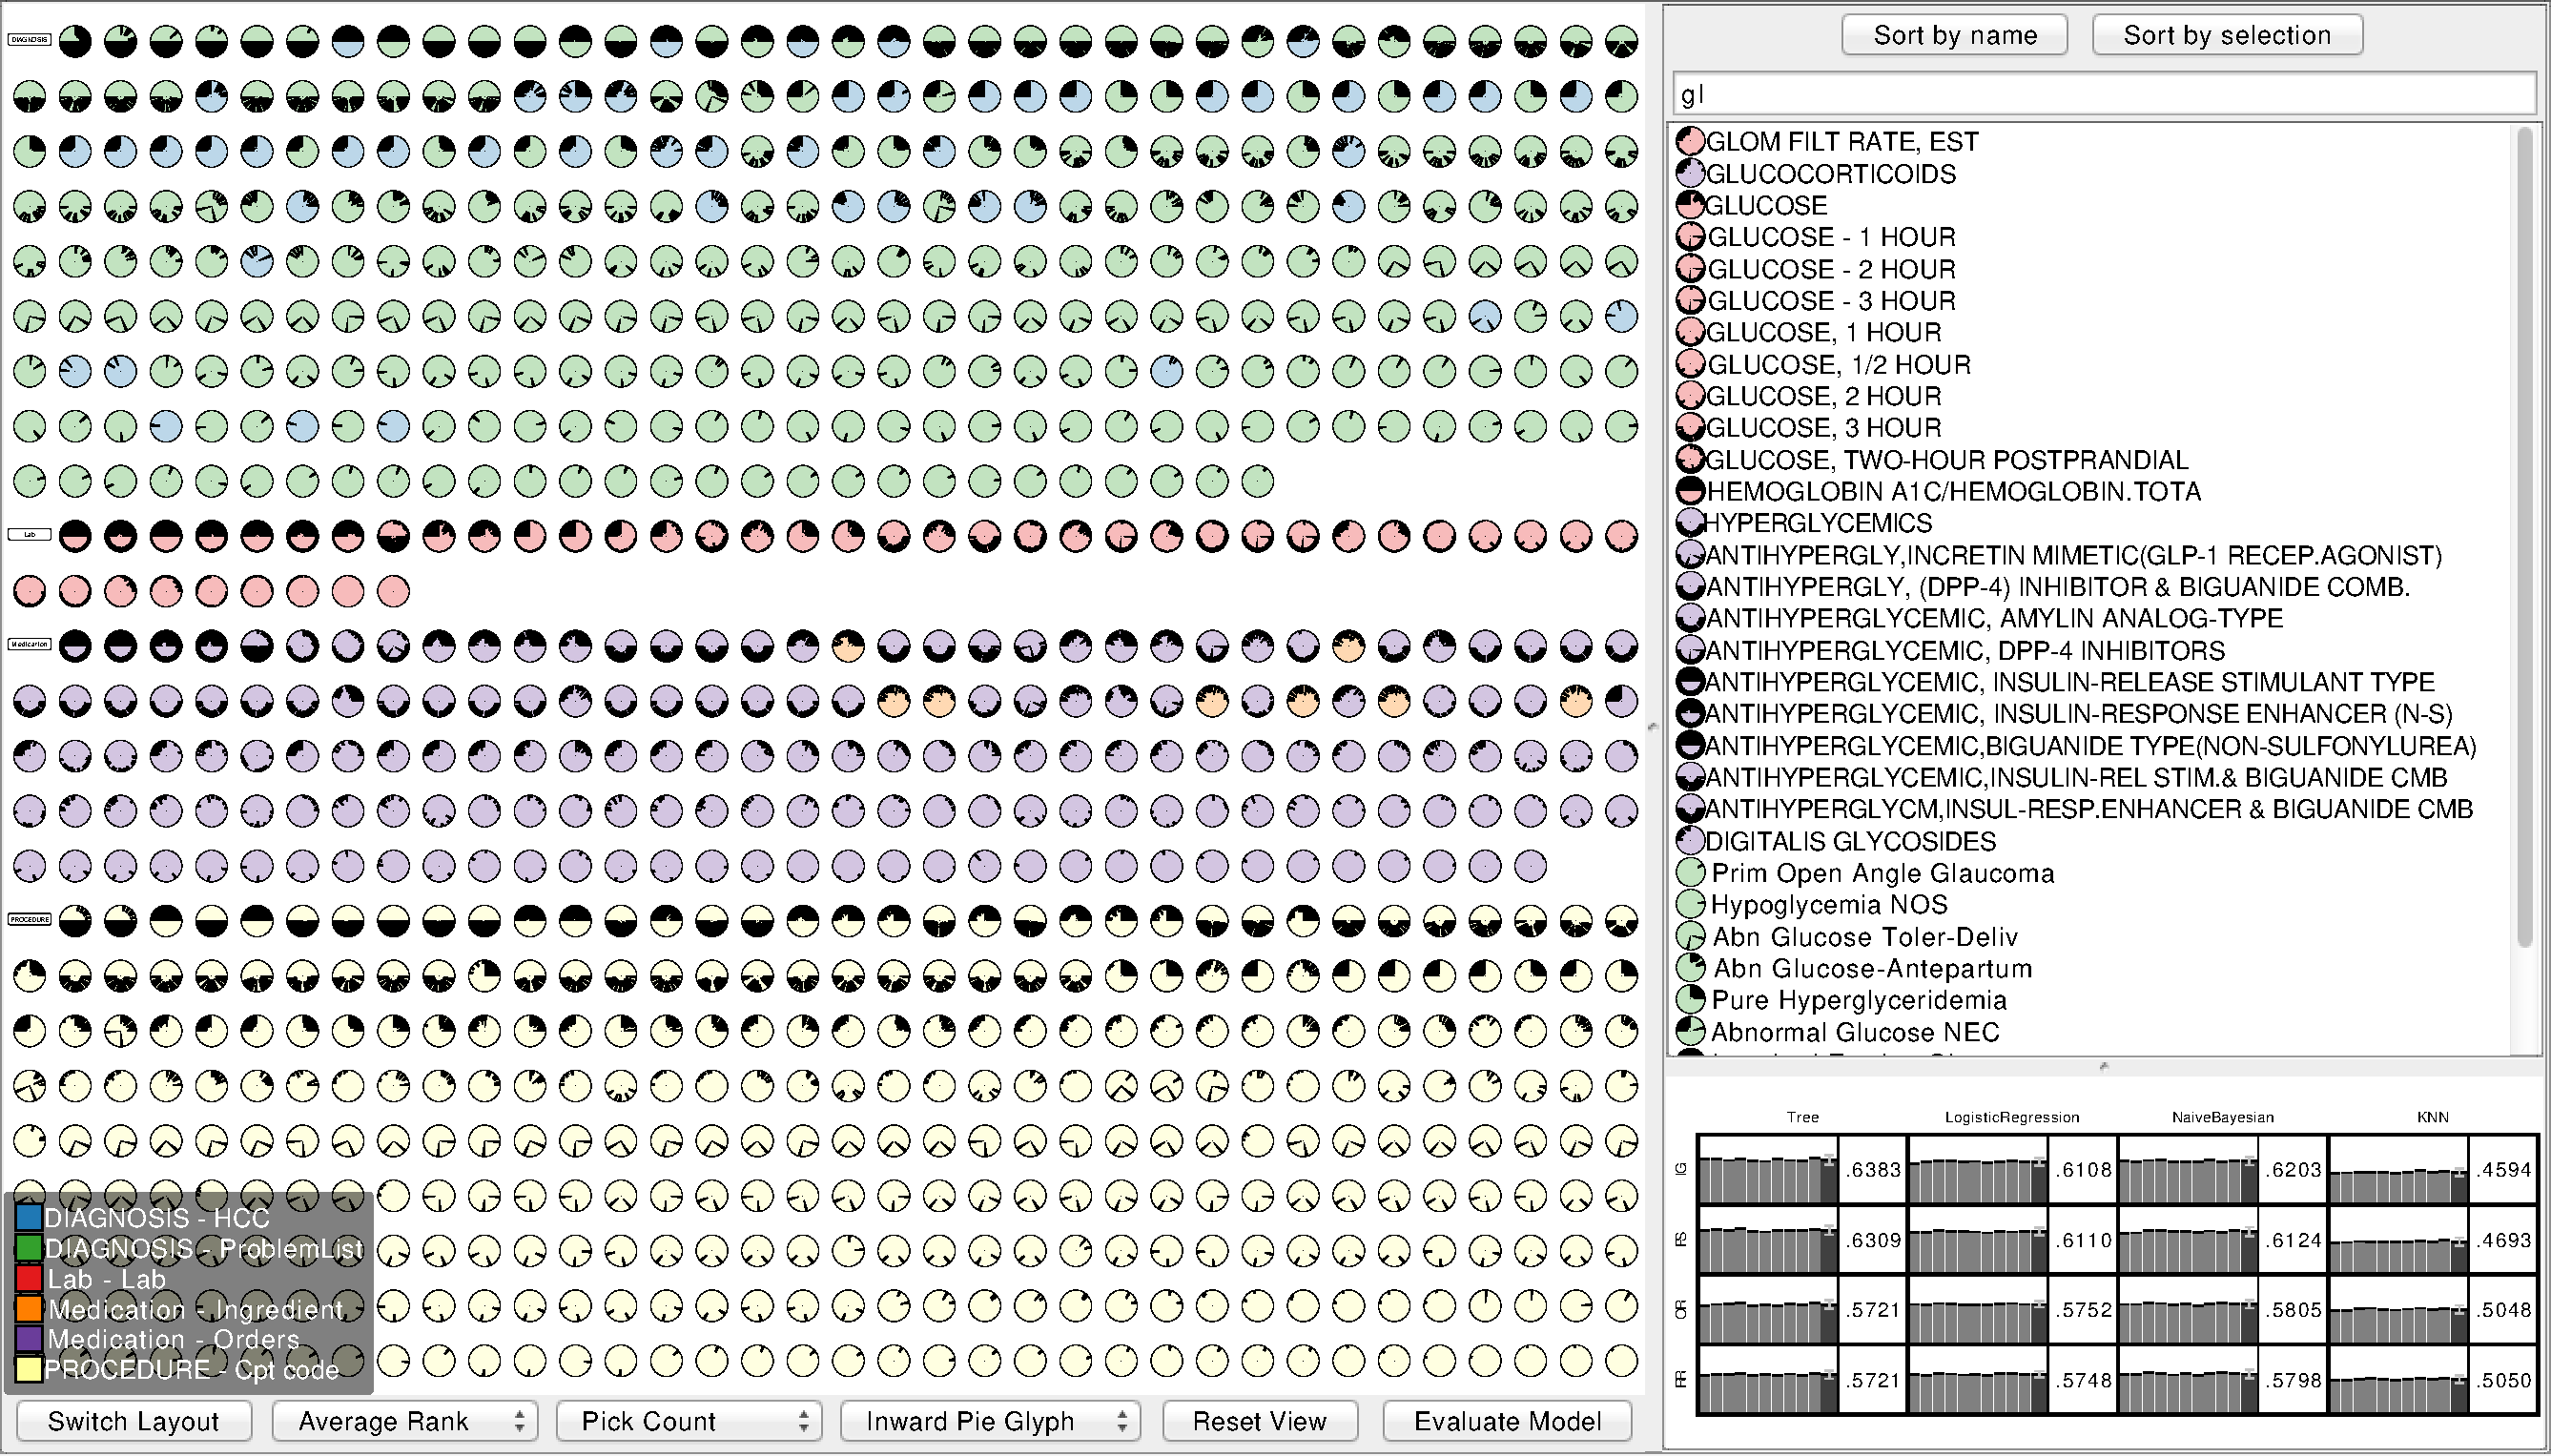
\includegraphics[width=\linewidth]{img/system}
% \caption{
% An overview of \infuse , a system for interactive feature selection.  On the left, the Feature View provides a way to visualize an overview of all features grouped by type and then sorted by importance.  The color key for the feature types and subtypes are shown at the bottom.  The buttons and combo boxes at the bottom can be used to switch layouts and define the axes of the scatter plot view shown in
% Figure~\ref{fig:scatter}.  On the top-right, the List View provides a sorted list of all features, useful for selections.
% This list can be filtered using the search box above. Currently only features containing the term ``gl" are shown.
% The remaining features are sorted by the number and position
% of the search term occurrences.
% On the bottom-right, the Classifier View (Figure~\ref{fig:classifier}) provides access to the quality scores of each model.  Users can also select features and build custom models with the Interactive Model Builder.
% }
% \label{fig:system}
% \end{figure}

% \subsection{List View}
% In addition to the aforementioned Feature View \infuse
% also shows a list containing all features using the same
% glyphs for easier recognition.
% This list can be sorted by name or the previously defined
% importance of a feature.
% When manually selected features are present they are
% grouped together at the top of the list and sorted as well.
% This allows for a quick overview of the selected features.
% Selection of features can be toggled by clicking on them in
% the List View.
% Above the List View is a search box
% in order to quickly find a specific feature or a group of
% features of a given subtype by name.

% \begin{figure}
% \centering
% 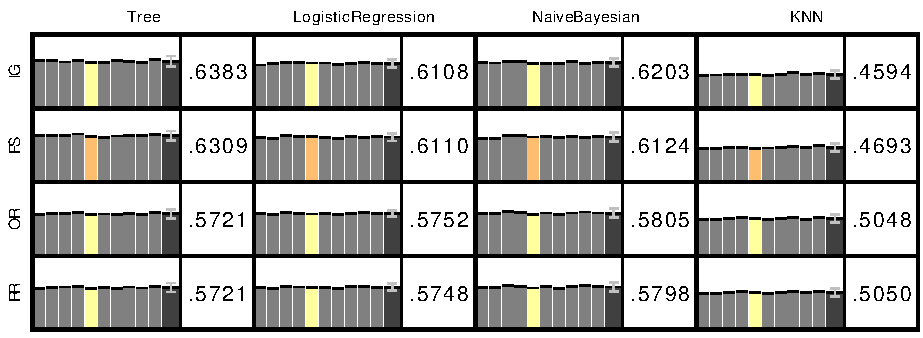
\includegraphics[width=\linewidth]{img/classifier}
% \caption{
% Classification results as shown in \infuse.
% Every column of the table represents one classification
% algorithm while each row displays the results of
% a feature selection algorithm.
% The results, in form of the area under curve (AUC) are
% shown as bar charts (one bar for every cross-validation fold
% and one bar showing the average AUC over all folds)
% as well as number (only the average AUC) in every cell.
% Selection highlights same folds under different algorithms.
% }
% \label{fig:classifier}
% \end{figure}

% \subsection{Classification View}
% In the third part of the tool, the Classification View shows
% the quality of the results of classification algorithms
% on the feature sets.
% The quality of those results are typically measured as area
% under curve (AUC) which is shown as bar charts in the table.
% Every row of the table shows the results for one feature selection
% algorithm and every column represents one classification
% algorithm, namely Decision Trees, Logistic Regression,
% Na\"ive Bayesian, or K-Nearest Neighbors.
% The bars show the results under a given cross-validation fold
% and the average AUC value, which is also displayed numerically.
% Error bars show the standard deviation of the AUC values across
% all folds.
% Clicking on a fold selects all features relevant for the given
% AUC in the Feature and List View and highlights bars showing
% the AUC for the same cross-validation fold under different
% algorithms.

% \subsection{Interactive Model Builder}
% The tool allows a user to select features in all three views.
% Those selected features can then be used as input to the
% classification algorithms creating a new row in the
% classification table. This enables experts to amend existing
% models by introducing their knowledge to it, potentially
% improving the results.

% \section{Conclusion}
% \infuse has been extensively used by researchers in the
% past, leading to several bug fixes in classification
% algorithms which were detected via unusual patterns in the
% feature glyph representation.
% Also, it revealed that different feature selection algorithms
% rank different features the highest
% (as seen in Figure~\ref{fig:infuse}) while ignoring features
% ranked high by other algorithms resulting in half-moon shaped
% glyphs. This could be explained with the high correlation of
% those features that are clinically similar.

% \chapter{Related Work}
% \label{chap:relwork}
% While using visual analytics for gaining insights into
% steps of the predictive modeling pipeline is a relatively
% unexplored topic, there exist some approaches for visualizing
% patient histories.
% \cite{10.1109/TVCG.2009.187}
% with \emph{LifeLines2} allows for comparing multiple patient
% histories at once by aligning them on a specific event.
% \cite{10.1109/TVCG.2013.200} group
% patients with the same order of events together and split
% into subgroups where the histories mismatch.
% This reduces the visual load on a user and makes finding
% common patterns easier.
% However, those approaches work only on a limited amount of
% different event types and when the histories are roughly similar
% in the data.

% For high dimensional data works mostly focus on the visualization
% of the data or the relationships within. \cite{Guo2003},
% for example shows feature similarity
% (\ie entropy and ${\chi}^2$) in a
% matrix and allows grouping of similar features.
% This can also be achieved with visual hierarchical
% dimension reduction
% (\cite{wang2003interactive}).
% This technique is based on a hierarchical clustering algorithm
% which clusters dimensions in terms of their similarity
% and presents them in a \textit{sunburst} visualization
% (\cite{yang2003interactive}).
% The level of aggregation can be interactively chosen
% and used to display data with the reduced set of dimensions.
% \cite{Johansson2009} present an
% integrated environment based on a \textit{parallel coordinates}
% visualization where the number and order of
% dimensions (axes) presented at any time is guided by
% a ranking algorithm that takes associations as well as
% intrinsic interestingness of each feature into account in
% order to interactively choose the number
% of features to visualize.
% Similar in spirit is the \textit{rank-by-feature}
% framework (\cite{seo2005rank}) in which
% data features are organized, ranked and visualized with
% 1D and 2D visual representations
% (\eg histograms, bar charts and scatterplots).
% Users can, for instance, inspect a matrix of feature pairs
% that is ranked by one of the available ranking
% functions and single out those features that show
% interesting associations.
% %A similar mechanism is also used in
% %\textit{scagnostics} (\cite{wilkinson2005graph}) a
% %quality metric approach (\cite{bertini2011quality}) that ranks
% %axis pairs according to the pattern/shape they create in
% %a scatterplot visualization.
% %
% %
% %
% %
% %More similar to the solution presented in this paper are visualizations that
% %focus on plotting dimensions as data points in the visual representation
% %(rather than, for example, as axes of a visualization where the data
% %items represent records of a data table).
% %\textit{Value and Relation Display} visualizes data features as icons
% %in a scatter plot visualization \cite{YangPHMWR04}.
% %The icons are positioned using a \textit{multidimensional scaling}
% %algorithm which positions dimensions with
% %similar distributions close together.
% %The icons are designed to represent the distribution of the
% %data values within the feature.
% %Such a display allows to detect groups of similar dimensions
% %and to construct multidimensional visualizations by subsetting
% %the original feature space.
% %\textit{Brushing Dimensions} \cite{Turkay2011} is a similar approach
% %where data features are plotted as dots in a scatter plot using
% %descriptive statistics as axes (e.g. variance, median, kurtosis).
% %The plot is paired with a data item scatter plot which allows for data
% %and feature linking and exploration.
% %
% %All of the methods described above are based on the calculation
% %of statistical parameters from the data as a way to characterize
% %and expose relationships between the features.
% %Our approach differs in that \systemname\ interacts directly
% %with feature selection and classification algorithms to help in
% %the discovery of predictive feature sets.
% %A similar approach is found in \textit{SmartStripes} \cite{May2011},
% %a visual analytics system that allows tight interaction between feature selection algorithms and visualization. Our system differs in that our focus is on the comparison of the output of multiple feature selection algorithms rather than a single one.

% Solutions more similar to \infuse are visualizations that
% plot features as data points rather than, for example, as axes
% of a scatter plot showing the data of those features as points.
% \cite{YangPHMWR04} shows features as icons in
% a scatter plot visualization. The positions are computed using
% a \textit{multidimensional scaling} algorithm putting features
% with similar data distributions close together.
% The icons represent the distribution of the data within the
% feature itself. This representation allows for easy creation
% of a feature subspace.
% A similar approach, \textit{Brushing Dimensions}
% (\cite{Turkay2011}), uses statistical
% features like variance, median, or kurtosis as potential axes
% for the scatter plot.
% A second scatter plot showing the actual data items which
% is linked to the feature scatter plot allows for in depth
% feature exploration.

% %%\joschi{\cite{Guo2003} interactive feature selection -- entropy matrix etc}
% %%\joschi{\cite{Ingram2010} creating workflow for feature reduction}
% %%\joschi{\cite{Johansson2009} interactive dim reduction via user defined weighting}
% %%\joschi{\cite{Kidwell2008} visualizing partially ranked data}
% %%\joschi{\cite{May2011} guiding fs with interactive system}
% %%\joschi{\cite{YangPHMWR04} features as points in scatterplot -- high dimension exploration -- MDS of correlation as layout}
% %%\joschi{\cite{Seo2005} rank by feature -- dendogram, scatterplot, matrix, list view}
% %%\joschi{\cite{Turkay2011} brushing dimensions}
% %
% %%\enrico{Other things we might want to include is subspace visualization as in a way it deal with the problem of finding feature subsets. E.g., Work from myself and from Wilkinson at VAST.}
% %%\joschi{PARAMO \cite{paramo}}
% %%\enrico{Should we briefly review feature selection strategies and algorithms as well?}

% %Visualization has also been used to aid in the creation of predictive models, not only in the selection of features that might be helpful in constructing such models. Visual construction and assessment of decision tree models have been the subject of a good number of works in the field. Ankerst \emph{et al.}, introduced the idea of using pixel-based visualization as a way to manually construct decision trees by giving the user the ability to observe class distributions within each node and to interactively select splitting points \cite{ankerst1999visual, ankerst2000towards}. A similar idea is proposed in \textit{PaintingClass} a visualization technique to manually build a decision tree through interaction of parallel coordinates and multidimensional scaling techniques to identify coherent groups of multidimensional data \cite{Teoh:2003:PIC:956750.956837}. More recently, \textit{BaobabView} has been presented as a system to inspect and validate a classification model through a tree representation. The paper presents a thorough analysis of the number of tasks that visualization can support in this area and how they are covered by the proposed system \cite{van2011baobabview}.
% %
% %While all the aforementioned systems focus largely on decision trees, visualization has been used in other classification and regression systems that leverage other prediction models. The \textit{iVisClassifier} \cite{choo2010ivisclassifier} for instance uses \textit{linear discriminant analysis (LDA)}, a supervised dimensionality reduction method, to project multidimensional data in a scatterplot visualization taking into account information provided by the data labels. The technique allows to visually link the high-dimensional structure to the low-dimensional representation and build clusters. The clusters are then used to classify new data that is progressively introduced into the system to refine the model. Steed \emph{et al.}, in their \textit{cyclone trend analysis} provide a parallel coordinates visualization that leverage computational analysis to identify features with high predictive power in stepwise regression tasks and allows to build predictive models for multidimensional climate data \cite{steed2009guided, steed2009tropical}. Recently, a visual analytics system for regression analysis has been proposed by M\"uhlbacher and Piringer \cite{muhlbacher2013partition}. The system is more similar to our work in nature as it also focuses on the predictive power of feature sets and guides the user in the predictive modeling process. The main difference between this work and ours is our focus on classification rather than regression models and the use of multiple feature selection and classification models to better understand how features score across multiple models.

% Interactive feature selection, as in
% \infuse , can also be found in \textit{SmartStripes}
% (\cite{May2011}) a visual analytics system
% guiding the manual creation of predictive feature sets.
% \cite{ankerst1999visual, ankerst2000towards}
% introduce the idea of using pixel-based visualization as a way to manually construct decision trees by giving the user the ability to observe class distributions within each node and to interactively select splitting points. A similar idea is proposed in \textit{PaintingClass} a visualization technique to manually build a decision tree through interaction of parallel coordinates and multidimensional scaling techniques to identify coherent groups of multidimensional data (\cite{Teoh:2003:PIC:956750.956837}).
% More recently, \textit{BaobabView} has been presented as a system to inspect and validate a classification model through a tree representation. The paper presents a thorough analysis of the number of tasks that visualization can support in this area and how they are covered by the proposed system (\cite{van2011baobabview}).
% \cite{muhlbacher2013partition} propose a visual analytics
% system for regression analysis.
% The system is more similar to \infuse in nature as it also
% focuses on the predictive power of feature sets
% and guides the user in the predictive modeling process.
% The main difference is, however, \infuse 's focus on
% classification rather that regression models and the use of
% multiple feature selection and classification models
% to better understand how features score across multiple models.

% \chapter{Conclusion and Future Work}
% \label{chap:conclusion}
% The two mentioned projects show how useful visual analytics
% can be in supporting predictive modeling.
% It improves and speeds up the work-flow of researchers and
% leads to new insights into their data and algorithms.
% However, there are several more projects thinkable to improve
% the work with the predictive modeling pipeline or
% clinical data in general:
% \begin{description}
% \item[Improving Patient Visualization]
%   The patient visualization in its current form shows only
%   the recorded events of the patient's history. This is
%   rather limiting given there are potentially many
%   factors responsible for the predicted diagnosis.
%   Many of which are present in the input data.
%   For example, the location of residency may have an
%   influence on diagnoses (think of John Snow's cholera map
%   of London) or whether relatives were diagnosed similarly.
%   Also, showing timelines of multiple patients at once
%   allowing to compare them and find patterns across a
%   set of patients is a challenging task.
%   This task could be solved by combining timelines visually
%   or by plotting patients as dots in a 2D space with a
%   suitable similarity metric in order to make finding
%   sets of patients with common patterns easier.
% \item[Cohort Construction]
%   The first part of the predictive modeling pipeline also
%   can be improved using visual analytics. Currently researchers
%   define case and control patient sets manually by looking
%   at the data. An interactive visual query system that provides
%   information about those sets can vastly improve
%   this task. Interesting information would be answering
%   the following questions:
%   ``\emph{Which events are present in only one/both set/s?}",
%   ``\emph{What is the gender, ethnicity, age,
%   \etc distribution of the patient sets?}", and
%   ``\emph{How do both sets compare in those attributes?}".
%   In addition to that, providing this information
%   at every point in the query a decision is made (\eg through
%   a filter) enables a user to reason about how the result
%   set will change when the query is altered.
%   This encourages experimenting with different queries via
%   trial and error and can lead to better patient cohorts.
% \item[Expanding Focus]
%   Patient timelines are not the only leverage point for
%   disease prediction and modeling.
%   For example cancer prediction using
%   human genomes could also benefit from visual analytics
%   in their predictive modeling process amending
%   on circus plots, a commonly used
%   visualization technique in this area.
%   Besides using different input data and solving
%   challenges arising from that, visual analytics can
%   improve handling high dimensional data or the
%   actual outcomes from feature selection and classification
%   algorithms.
%   For example, correlations between features currently
%   is not represented in \infuse .
%   A view showing correlations between features mapped to
%   distances can help finding redundant features thus
%   manually improving feature selection algorithms and
%   increasing their overall performance.
% \end{description}
% %
% %For example, it is thinkable to improve the definition of
% %cohort patient sets by utilizing a visual query system.
% %Also, results from the aforementioned projects can
% %be applied in other domains as well.
% %Especially, using visual analytics for debugging algorithms
% %is an under utilized application.
% %
% %Additionally, the current projects have room for improvements. For example,
% %the patient timeline visualization can be improved by including more information
% %about the patients, \eg labeling time ranges when a patient was not insured by the given data provider to distinguish
% %times when the patient didn't see a doctor from simply
% %missing data, or incooperating the region of residency
% %into the tool to explore regionally dependent diseases.
% %Also, this visualization can be extended
% %to show multiple patients at once.
% %
% %Further future tasks are integrating the projects even more
% %into the researchers' work-flow allowing them to use the
% %tools in their full potential and providing
% %valuable feedback and feature requests.
